\باب{سمتی میدان میں تکمل}\شناخت{باب_سمتی_میدان_میں_تکمل}
\موٹا{ایک جائزہ}\quad
اس باب  کا موضوع  سمتی میدان میں تکمل ہے۔ اس باب کی ریاضی کو برقناطیسیت  کے خواص   بیان کرنے کے لئے، تاروں میں حرارت  کے بہاو پر غور ، اور  مصنوعی سیارہ کو  مدار میں منتقل کرنے  کے لئے درکار توانائی کے حصول کے لئے استعمال کیا جاتا ہے۔

\حصہ{لکیری تکمل}
جب فضا میں  تفاعل \عددی{f(x,y,z)} کے دائرہ کار سے منحنی \عددی{\kvec{r}(t)=g(t)\ai+h(t)\aj+k(t)\ak,\,a\le t\le b}  گزرے تب اس   منحنی  کے ساتھ چلتے ہوئے \عددی{f}  کی قیمتیں مرکب تفاعل \عددی{f(g(t),h(t),k(t))} دیگا۔ نقطہ \عددی{a} سے \عددی{b} تک لمبائی قوس  کے لحاظ سے اس مرکب تفاعل کے تکمل کو قوس کے ساتھ \عددی{f} کا  \اصطلاح{لکیری  تکمل}\فرہنگ{تکمل!لکیری}\حاشیہب{line integral}\فرہنگ{integral!line} کہتے ہیں۔  تین بعدی جیومیٹری کے باوجود،  لکیری تکمل حقیقی اعداد کے وقفہ پر حقیقی قیمت تفاعل کا سادہ تفاعل ہو گا۔

لکیری تکمل کی اہمیت اس کے استعمال میں ہے۔ ان تکملات  کی مدد سے ہم  متغیر قوتوں کی فضا میں راہ پر کام    اور قوس  کے ساتھ یا  سرحد پار کرتی سیال کی شرح بہاو  کا حساب کرتے ہیں۔

\begin{figure}
\centering
\begin{tikzpicture}[font=\small,declare function={fx(\x)=sin(\x)+1/3*cos(3*\x);fy(\t)=cos(\t);fz(\t)=\t/100;}]
\coordinate (O) at (-0.5,-1);
\draw[smooth, domain=5:120]plot ({\x/30},{fx(\x)});
\foreach \t in {1,3.2,4.6,7,9,11}{\path[| mark=0.5] ({(\t-0.1)/3},{fx((\t-0.1)*10)}) -- ({(\t+0.1)/3},{fx((\t+0.1)*10)});}
\draw[] ({7.5/3},{fx(7.5*10)})node[circ]{}node[right,yshift=-1ex]{$(x_k,y_k,z_k)$};
\draw[-stealth](O)--++(-0.5,-0.5)node[left]{$x$};
\draw[-stealth](O)--++(3,0)node[right]{$y$};
\draw[-stealth](O)--++(0,2)node[left]{$z$};
\draw[-latex](O)--({4/3},{fx(4*10)})node[pos=0.5,below]{$\kvec{r}$};
\draw[] ({1/3},{fx(1*10)})node[xshift=-2ex,yshift=2ex]{$t=a$};
\draw[] ({11/3},{fx(11*10)})node[xshift=2ex,yshift=2ex]{$t=b$};
\draw[decorate,decoration={brace,amplitude=5pt, raise=5pt}] ({7/3},{fx(7*10)})--({9/3},{fx(9*10)})node[above left,shift={(145:5pt)}]{$\Delta s_k$};
\end{tikzpicture}
\caption{
منحنی \عددی{\kvec{r}=g(t)\ai+h(t)\aj+k(t)\ak} کو \عددی{t=a} اور \عددی{t=b} کے بیچ قوسچوں میں تقسیم کیا گیا ہے۔ ایک علامتی  قوسچہ کی لمبائی \عددی{\Delta s_k} ہے۔
}
\label{شکل_کثیر_قوسچہ}
\end{figure}

\جزوحصہء{تعریفات اور  علامتیت}
فرض کریں تفاعل \عددی{f(x,y,z)}  کے  دائرہ کار میں منحنی \عددی{\kvec{r}(t)=g(t)\ai+h(t)\aj+k(t)\ak,\,a\le t\le b} پائی جاتی ہے۔ ہم اس منحنی کی،  متناہی تعداد کی  قوسچوں میں، خانہ بندی کرتے ہیں (شکل \حوالہ{شکل_کثیر_قوسچہ})۔ ایک علامتی قوسچہ کی لمبائی \عددی{\Delta s_k} ہو گی۔ ہم ہر قوسچہ پر  ایک نقطہ \عددی{(x_k,y_k,z_k)}  منتخب کر کے درج ذیل مجموعہ لیتے ہیں۔
\begin{align}\label{مساوات_میدان_خطی_تکمل_الف}
J_n=\sum\limits_{k=1}^{n} f(x_k,y_k,z_k)\Delta s_k
\end{align}
اگر \عددی{f} استمراری ہو اور \عددی{g}، \عددی{h}،  اور \عددی{k} کے  اول تفرقات استمراری ہوں تب جیسے جیسے  \عددی{n} بڑھایا جائے، \عددی{\Delta s_k}  صفر تک پہنچے گی اور   مساوات \حوالہ{مساوات_میدان_خطی_تکمل_الف} کا مجموعہ  ایک حد کو پہنچے گا۔ ہم اس حد کو \اصطلاح{ \عددی{a} تا \عددی{b} اس قوس پر \عددی{f} کا تکمل} کہتے ہیں۔  قوس کو \عددی{C} سے ظاہر کرتے ہوئے  اس تکمل کو علامتی طور پر درج ذیل لکھا جاتا ہے۔
\begin{align}\label{مساوات_میدان_خطی_تکمل_ب}
\int_C f(x,y,z)\dif s\quad \quad \text{\RL{"\عددی{C} پر \عددی{f} کا تکمل"}}
\end{align}

\جزوحصہء{ہموار منحنیات پر تکمل کی قیمت کا حصول}
اگر وقفہ \عددی{a\le t\le b} پر \عددی{\kvec{r}(t)} ہموار ہو   (\عددی{\kvec{v}=\tfrac{\dif\kvec{r}}{\dif t}}   استمراری  ہو اور کبھی بھی \عددی{\kvec{0}} نہ ہو)   تب ہم \عددی{\dif s}  کو بیان کرنے کے لئے درج ذیل مساوات استعمال کر سکتے ہیں  چونکہ  اس سے \عددی{\dif s=\abs{\kvec{v}(\tau)}\dif t} لکھا جا سکتا ہے۔
\begin{align*}
s(t)=\int_a^t \abs{\kvec{v}(\tau)} \dif \tau\quad\text{\small\RL{حصہ \حوالہ{حصہ_سمتی_تفاعل_لمبائی_قوس_اور_اکائی_سمتیہ} کی  مساوات \حوالہ{مساوات_سمتی_تفاعل_لمبائی_قوس_ت} میں \عددی{t_0=a}}}
\end{align*}
اعلٰی احصاء کا ایک مسئلہ کہتا ہے کہ ایسی صورت میں ہم  درج ذیل طریقہ سے \عددی{C} پر \عددی{f} کے تکمل کی قیمت حاصل کر  سکتے ہیں۔
\begin{align*}
\int_C f(x,y,z)\dif s=\int_a^b f(g(t),h(t),k(t))\abs{\kvec{v}(t)}\dif t
\end{align*} 
ہم جس مقدار معلوم روپ کو بھی استعمال کریں، جب تک زیر استعمال مقدار معلوم   روپ ہموار ہو، یہ کلیہ ہمیں تکمل کی قیمت دیگا۔ 

\جزوحصہء{لکیری تکمل کی قیمت کا حصول}
منحنی  \عددی{C} پر استمراری تفاعل \عددی{f} کا  تکمل لینے کے لئے
\begin{enumerate}[a.]
\item
\عددی{C} کی مقدار معلوم روپ تلاش کریں:
\[\kvec{r}(t)=g(t)\ai+h(t)\aj+k(t)\ak,\quad a\le t\le b\]
\item
درج ذیل تکمل کی قیمت حاصل کریں۔
\begin{align}\label{مساوات_میدان_خطی_تکمل_پ}
\int_Cf(x,y,z)\dif s=\int_a^bf(g(t),h(t),k(t))\abs{\kvec{v}(t)}\dif t
\end{align}
\end{enumerate}

دھیان رہے کہ مستقل تفاعل \عددی{f=1} کی صورت میں مذکورہ بالا تکمل \عددی{C} کی لمبائی دیگا۔

%====================
\ابتدا{مثال}\شناخت{مثال_میدان_راہ_الف}
مبدا سے  نقطہ \عددی{(1,1,1)} تک قطع پر \عددی{f(x,y,z)=x-3y^2+z} تکمل کریں (شکل \حوالہ{شکل_مثال_میدان_راہ_الف})۔

حل:\quad
ہم  ذہن میں آنے والا سادہ ترین مقدار معلوم روپ استعمال کرتے ہیں
\[\kvec{r}(t)=t\ai+t\aj+t\ak,\quad 0\le t\le 1\]
جس کی اجزاء کے اول تفرقات استمراری ہیں اور \عددی{\abs{\kvec{v}(t)}=\sqrt{1^2+1^2+1^2}=\sqrt{3}} کبھی بھی \عددی{\kvec{0}} نہیں ہو سکتا ہے لہٰذا  یہ مقدار معلوم روپ ہموار ہے۔ یوں   \عددی{C} پر \عددی{f} کا تکمل درج ذیل ہو گا۔
\begin{align*}
\int_C f(x,y,z)\dif s&=\int_0^1 f(t,t,t)(\sqrt{3})\dif t&&\text{\RL{مساوات \حوالہ{مساوات_میدان_خطی_تکمل_پ}}}\\
&=\int_0^1 (t-3t^2+t)\sqrt{3}\dif t\\
&=\sqrt{3}\int_0^1 (2t-3t^2)\dif t=\sqrt{3}\big[t^2-t^3\big]_0^1=0
\end{align*} 
\انتہا{مثال}
%===================
\begin{figure}
\centering
\begin{minipage}{0.45\textwidth}
\centering
\begin{tikzpicture}[]
\begin{axis}[clip=false,view/h=110,small,axis lines=middle,xtick={\empty},ytick={\empty},ztick={\empty},enlargelimits=true, xlabel={$x$}, ylabel={$y$},zlabel={$z$}, xlabel style={anchor=north},ylabel style={anchor=west},zlabel style={anchor=south},colormap={}{gray(0cm)=(0.6);gray(1cm)=(0.9);}]
\addplot3[]plot coordinates {(0,0,0)(1,1,1)}node[pos=1,circ]{}node[pos=1,right]{$(1,1,1)$}node[pos=0.5,above]{$C$};
\addplot3[dashed]plot coordinates {(1,1,1)(1,1,0)(0,0,0)};
\addplot3[]plot coordinates {(1,1,0)}node[right]{$(1,1,0)$};
\end{axis}
\end{tikzpicture}
\caption{تکمل کی راہ (مثال \حوالہ{مثال_میدان_راہ_الف})۔}
\label{شکل_مثال_میدان_راہ_الف}
\end{minipage}\hfill
\begin{minipage}{0.45\textwidth}
\centering
\begin{tikzpicture}[]
\begin{axis}[clip=false,view/h=110,small,axis lines=middle,xtick={\empty},ytick={\empty},ztick={\empty},enlargelimits=true, xlabel={$x$}, ylabel={$y$},zlabel={$z$}, xlabel style={anchor=north},ylabel style={anchor=west},zlabel style={anchor=south},colormap={}{gray(0cm)=(0.6);gray(1cm)=(0.9);},zmax=0.75]
\addplot3[]plot coordinates {(0,0,0)(1,1,0)}node[pos=0,circ]{}node[pos=0,pin=135:{$(0,0,0)$}]{}node[pos=1,circ]{}node[pos=1,right]{$(1,1,0)$}node[pos=0.5,below]{$C_1$};
\addplot3[]plot coordinates {(1,1,0)(1,1,1)}node[pos=1,circ]{}node[pos=1,right]{$(1,1,1)$}node[pos=0.75,right]{$C_2$};
\end{axis}
\end{tikzpicture}
\caption{تکمل کی راہ (مثال \حوالہ{مثال_میدان_راہ_ب})۔}
\label{شکل_مثال_میدان_راہ_ب}
\end{minipage}
\end{figure}


\جزوحصہ{جمع پذیری}
  اگر متناہی تعداد کی منحنیات \عددی{C_1}، \عددی{C_2}، \نقطے، \عددی{C_n} کو ایک دوسرے کے ساتھ جوڑ کر منحنی \عددی{C} حاصل کی جائے تب  \عددی{C} پر تفاعل کا تکمل ان منحنیات پر تفاعل کے تکملات کا مجموعہ ہو گا:
\begin{align}\label{مساوات_میدان_خطی_تکمل_ت}
\int_C f\dif s=\int_{C_1} f\dif s+\int_{C_2} f\dif s+\cdots+\int_{C_n} f\dif s
\end{align}

\ابتدا{مثال}\شناخت{مثال_میدان_راہ_ب}
مبدا سے نقطہ \عددی{(1,1,1)} تک  راہ \عددی{C_1} اور \عددی{C_2}  پر چل کر پہنچا جاتا ہے (شکل \حوالہ{شکل_مثال_میدان_راہ_ب})۔ یوں \عددی{C} ان کا اشتراک \عددی{C_1\cup C_2} ہو گا۔ تفاعل \عددی{f(x,y,z)=x-3y^2+z}  کے تکمل کی قیمت  \عددی{C_1\cup C_2} پر  تلاش کریں۔

حل:\quad
ہم \عددی{C_1} اور \عددی{C_2} کے لئے،  ذہن میں آنے  والے  سادہ ترین،  مقدار معلوم روپ  استعمال کرتے ہیں:
\begin{align*}
C_1:\quad \kvec{r}(t)&=t\ai+t\aj,\, 0\le t\le 1;\, \abs{\kvec{v}}=\sqrt{1^2+1^2}=\sqrt{2}\\
C_2:\quad \kvec{r}(t)&=\ai+\aj+t\ak,\, 0\le t\le 1;\, \abs{\kvec{v}}=\sqrt{0^2+0^2+1^2}=1
\end{align*}
ان مقدار معلوم روپ کے ساتھ درج ذیل حاصل ہو گا۔
\begin{align*}
\int_{C_1\cup C_2}f(x,y,z)\dif s&=\int_{C_1}f(x,y,z)\dif s+\int_{C_2}f(x,y,z)\dif s&&\text{\RL{مساوات \حوالہ{مساوات_میدان_خطی_تکمل_ت}}}\\
&=\int_0^1 f(t,t,0)\sqrt{2} \dif t+\int_0^1 f(1,1,t)(1)\dif t\\
&=\int_0^1 (t-3t^2+0)\sqrt{2}\dif t+\int_0^1(1-3+t)(1)\dif t\\
&=\sqrt{2}\big[\frac{t^2}{2}-t^3\big]_0^1+\big[\frac{t^2}{2}-2t\big]_0^1=-\frac{\sqrt{2}}{2}-\frac{3}{2}
\end{align*}
\انتہا{مثال}
%=======================

یہاں   مثال \حوالہ{مثال_میدان_راہ_الف} اور مثال \حوالہ{مثال_میدان_راہ_ب} کے نتائج پر غور کرتے ہیں۔اول، دیکھیں کہ  موزوں منحنی کے اجزاء \عددی{f} میں پر کرتے ہی  \عددی{t} کے لحاظ سے ایک  سادہ تکمل حاصل ہوتا ہے۔ دوم،  \عددی{C_1\cup C_2} پر \عددی{f} کا تکمل لینے کے لئے \عددی{C_1} اور \عددی{C_2} پر \عددی{f} کے علیحدہ علیحدہ تکملات لے کر نتائج  کا مجموعہ لیا جاتا ہے۔سوم،      مثال \حوالہ{مثال_میدان_راہ_الف} میں \عددی{C}  اور مثال \حوالہ{مثال_میدان_راہ_ب} میں \عددی{C_1\cup C_2} پر تکمل کے نتائج ایک دوسرے سے مختلف تھے۔ عموماً تفاعل کے لئے دو نقطوں کے بیچ مختلف راہ پر تکملات کے نتائج ایک دوسرے سے مختلف ہوں گے۔ البتہ بعض تفاعل کے لئے تکمل کی قیمت پر راہ کا کوئی اثر نہیں ہوتا ہے۔

\جزوحصہء{کمیت اور معیار اثر کا حساب}
ہم اسپرنگ اور تار کو فضا میں ہموار منحنی پر  استمراری کمیتی کثافت \عددی{\delta(x,y,z)} کی تقسیم تصور کرتے ہیں۔ یوں اسپرنگ یا تار کی کمیت، مرکز کمیت، اور ان کے معیار اثر اور  رداس دوار کا حساب    درج ذیل  کلیات سے کیا جائے گا۔ یہی کلیات باریک (پتلی) تار کے لئے بھی کارآمد ہوں گے۔
\begin{description}
\item{کیمت:}\quad
\(M=\iiint\limits_D \delta(x,y,z) \dif H\)
\item{محددی مستویات کے لحاظ سے اول معیار اثر:}
\[M_{yz}=\int_C x\delta \dif s,\quad M_{xz}=\int_C y\delta \dif s,\quad M_{xy}=\int_Cz\delta \dif s\]
\item{مرکز کمیت کے محدد:}
\[\bar{x}=\frac{M_{yz}}{M},\quad \bar{y}=\frac{M_{xz}}{M},\quad \bar{z}=\frac{M_{xy}}{M}\]
\item{معیار اثر:}
\begin{align*}
I_x&=\int_C(y^2+z^2)\delta \dif s & I_y&=\int_C(x^2+z^2)\delta \dif s\\
I_z&=\int_C(x^2+y^2)\delta \dif s& I_L&=\int_C r^2\delta \dif s
\end{align*}
جہاں  لکیر \عددی{L} سے نقطہ \عددی{(x,y,z)} تک فاصلہ \عددی{r(x,y,z)} ہے۔
\item{لکیر \عددی{L} کے لحاظ سے رداس دور:}\quad
\(R_L=\sqrt{\frac{I_L}{M}}\)
\end{description}

%==================================
\ابتدا{مثال}\شناخت{مثال_سمتی_تکمل_اسپرنگ}
ایک اسپرنگ درج ذیل پیچدار منحنی کے ساتھ ساتھ پایا جاتا ہے (شکل \حوالہ{شکل_مثال_سمتی_تکمل_اسپرنگ})۔
\[\kvec{r}(t)=(\cos t)\ai+(\sin t)\aj+t\,\ak,\quad 0\le t\le 2\pi\]
اس اسپرنگ کی کثافت مستقل تفاعل \عددی{\delta=1} ہے۔ اس اسپرنگ کی کمیت اور مرکز کمیت  اور محور \عددی{z} کے لحاظ سے   جمودی معیار اثر اور رداس دوار معلوم کریں۔

حل:\quad
ہم اسپرنگ کا خاکہ بناتے ہیں۔ تشاکلی کی بنا اس کا مرکز کمیت محور \عددی{z} پر  نقطہ \عددی{(0,0,\pi)} پر پایا جائے گا۔  باقی حساب کے لئے ہم \عددی{\abs{\kvec{v}(t)}} تلاش کرتے ہیں:
\begin{align*}
\abs{\kvec{v}(t)}&=\sqrt{\big(\frac{\dif x}{\dif t}\big)^2+\big(\frac{\dif y}{\dif t}\big)^2+\big(\frac{\dif z}{\dif t}\big)^2}\\
&=\sqrt{(-4\sin 4t)^2+(4\cos 4t)^2+1}=\sqrt{17}
\end{align*}
اب مذکورہ بالا کلیات استعمال کرتے ہوئے درج ذیل حاصل ہو گا۔
\begin{align*}
M&=\int\limits_{\text{پیچدار}} \delta \dif s=\int_0^{2\pi} (1)\sqrt{17}\dif t=2\pi\sqrt{17}\\
I_z&=\int\limits_{\text{پیچدار}} (x^2+y^2)\delta \dif s=\int_0^{2\pi}(\cos^2 4t+\sin^2 4t)(1)(\sqrt{17})\dif t\\
&=\int_0^{2\pi}\sqrt{17}\dif t=2\pi\sqrt{17}\\
R_z&=\sqrt{\frac{I_z}{M}}=\sqrt{\frac{2\pi\sqrt{17}}{2\pi\sqrt{17}}}=1
\end{align*}
دھیان رہے کہ محور \عددی{z} کے لحاظ سے رداس دوار عین اس بیلن کے رداس  جتنا ہے جس پر اسپرنگ لپیٹا گیا ہے۔
\انتہا{مثال}
%=====================

\begin{figure}
\centering
\begin{minipage}{0.45\textwidth}
\centering
\begin{tikzpicture}[declare function={fx(\t)=cos(deg(4*\t));fy(\t)=sin(deg(4*\t));fz(\z)=\t;}]
\begin{axis}[clip=false,view/h=110,small,axis lines=middle,xtick={1},ytick={\empty},ztick={pi,2*pi},zticklabels={$\pi$,$2\pi$},enlargelimits=true, xlabel={$x$}, ylabel={$y$},zlabel={$z$}, xlabel style={anchor=east},ylabel style={anchor=west},zlabel style={anchor=west},colormap={}{gray(0cm)=(0.6);gray(1cm)=(0.9);}]
\addplot3[domain=0:2*pi,variable=\t,samples y=0,samples=100]({fx(t)},{fy(t)},{fz(t)});
\addplot3[]plot coordinates {(0,0,pi)}node[circ]{};
\end{axis}
\end{tikzpicture}
\caption{اسپرنگ برائے مثال \حوالہ{مثال_سمتی_تکمل_اسپرنگ}}
\label{شکل_مثال_سمتی_تکمل_اسپرنگ}
\end{minipage}\hfill
\begin{minipage}{0.45\textwidth}
\centering
\begin{tikzpicture}[declare function={fy(\t)=cos(deg(\t));fz(\t)=sin(deg(\t));}]
\begin{axis}[clip=false,view/h=110,small,axis lines=middle,xtick={\empty},ytick={-1,1},ztick={0.57,1},zticklabels={$0.57$,$1$},enlargelimits=true, xlabel={$x$}, ylabel={$y$},zlabel={$z$}, xlabel style={anchor=east},ylabel style={anchor=west},zlabel style={anchor=south},colormap={}{gray(0cm)=(0.6);gray(1cm)=(0.9);},]
\addplot3[domain=0:pi,variable=\t,samples y=0,smooth]({0},{fy(t)},{fz(t)});
\addplot3[]plot coordinates {(0.1,0,0)}node[right,xshift=2ex]{$y^2+z^2=1,\, z\ge 0$};
\addplot3[]plot coordinates {(0,0,0.57)}node[circ]{};
\end{axis}
\end{tikzpicture}
\caption{محراب کا مرکز کمیت (مثال \حوالہ{مثال_سمتی_تکمل_قوس_کی_کمیت})۔}
\label{شکل_مثال_سمتی_تکمل_قوس_کی_کمیت}
\end{minipage}
\end{figure}
\ابتدا{مثال}\شناخت{مثال_سمتی_تکمل_قوس_کی_کمیت}
مستوی \عددی{yz} میں نصف دائرہ \عددی{y^2+z^2=1,\, z\ge 0} پر ایک  دبلا پتلا محراب پایا جاتا ہے (شکل \حوالہ{شکل_مثال_سمتی_تکمل_قوس_کی_کمیت})۔ محراب کے نقطہ \عددی{(x,y,z)} پر کثافت \عددی{\delta(x,y,z)=2-z} ہے۔ محراب کا مرکز کمیت تلاش کریں۔

حل:\quad
چونکہ یہ  محراب مستوی \عددی{yz} میں پایا جاتا ہے  اور محور \عددی{z} کے لحاظ سے اس کی کمیتی تقسیم دونوں اطراف یکساں ہے   لہٰذا \عددی{\bar{x}=0} اور \عددی{\bar{y}=0} ہوں گے۔ہم دائرہ کی مقدار معلوم روپ
\[\kvec{r}(t)=(\cos t)\aj+(\sin t)\ak,\, 0\le t\le \pi\]
 لکھتے ہوئے \عددی{\bar{z}} دریافت کرتے ہیں۔اس مقدار معلوم روپ کے لئے
\[\abs{\kvec{v}(t)}=\sqrt{\big(\frac{\dif x}{\dif t}\big)^2+\big(\frac{\dif y}{\dif t}\big)^2+\big(\frac{\dif z}{\dif t}\big)^2}=\sqrt{(0)^2+(-\sin t)^2+(\cos t)^2}=1\]
ہو گا۔ یوں مذکورہ بالا کلیات استعمال کرتے ہوئے درج ذیل ہو گا۔
\begin{align*}
M&=\int_C \delta \dif s=\int_C (2-z)\dif s=\int_0^{\pi}(2-\sin t)\dif t=2\pi-2\\
M_{xy}&=\int_0^C z\delta \dif s=\int_C z(2-z)\dif s=\int_0^{\pi} (\sin t)(2-\sin t)\dif t\\
&=\int_0^{\pi} (2\sin t-\sin^2 t)\dif t=\frac{8-\pi}{2}\\
\bar{z}&=\frac{M_{xy}}{M}=\frac{8-\pi}{2}\cdot\frac{1}{2\pi-2}\approx 0.57
\end{align*}
یوں مرکز کمیت تقریباً \عددی{(0,0,0.57)} ہو گا۔
\انتہا{مثال}
%==================

\جزوحصہء{سوالات}
\ابتدا{سوالات}
\موٹا{سمتی مساوات کی ترسیمات}\\
سوال \حوالہ{سوال_سمتی_تکمل_مساوات_ترسیم_الف} تا سوال \حوالہ{سوال_سمتی_تکمل_مساوات_ترسیم_چ} میں دی گئی مساوات کی مطابقتی ترسیم شکل \حوالہ{شکل_سوال_سمتی_تکمل_مساوات_ترسیم_پ} تا شکل \حوالہ{شکل_سوال_سمتی_تکمل_مساوات_ترسیم_ت} میں تلاش کریں۔
\begin{figure}
\centering
\begin{minipage}{0.22\textwidth}
\centering
\begin{tikzpicture}[declare function={fx(\t)=2*cos(deg(\t));fy(\t)=2*sin(deg(\t));fz(\t)=0;}]
\begin{axis}[clip=false,width=4cm, font=\tiny,view/h=120,axis lines=middle,xtick={2},ytick={2},ztick={\empty},enlargelimits=true, xlabel={$x$}, ylabel={$y$},zlabel={$z$}, xlabel style={anchor=east},ylabel style={anchor=west},zlabel style={anchor=south},colormap={}{gray(0cm)=(0.6);gray(1cm)=(0.9);},xmax=2.25,ymax=2.125]
\addplot3[domain=0:2*pi,variable=\t,samples y=0,->-=0.2]({fx(t)},{fy(t)},{fz(t)});
\end{axis}
\end{tikzpicture}
\caption{}
\label{شکل_سوال_سمتی_تکمل_مساوات_ترسیم_پ}
\end{minipage}\hfill
\begin{minipage}{0.22\textwidth}
\centering
\begin{tikzpicture}[declare function={fx(\t)=0;fy(\t)=(\t^2-1);fz(\t)=2*\t;}]
\begin{axis}[clip=false,width=4cm, font=\tiny,view/h=120,axis lines=middle,xtick={\empty},ytick={-1},ztick={-2,2},enlargelimits=true, xlabel={$x$}, ylabel={$y$},zlabel={$z$}, xlabel style={anchor=east},ylabel style={anchor=west},zlabel style={anchor=south},colormap={}{gray(0cm)=(0.6);gray(1cm)=(0.9);},zmin=-2.5,zmax=2.5]
\addplot3[domain=-1:1,variable=\t,samples y=0,->-=0.25]({fx(t)},{fy(t)},{fz(t)})node[pos=0,circ]{}node[pos=1,circ]{};
\end{axis}
\end{tikzpicture}
\caption{}
\label{شکل_سوال_سمتی_تکمل_مساوات_ترسیم_ج}
\end{minipage}\hfill
\begin{minipage}{0.22\textwidth}
\centering
\begin{tikzpicture}[declare function={fx(\t)=\t;fy(\t)=1-\t;fz(\t)=0;}]
\begin{axis}[clip=false,width=4cm, font=\tiny,view/h=110,axis lines=middle,xtick={1},ytick={1},ztick={\empty},enlargelimits=true, xlabel={$x$}, ylabel={$y$},zlabel={$z$}, xlabel style={anchor=east},ylabel style={anchor=west},zlabel style={anchor=south},colormap={}{gray(0cm)=(0.6);gray(1cm)=(0.9);},xmax=1.25,ymax=1.125]
\addplot3[domain=0:1,variable=\t,samples y=0,->-=0.5]({fx(t)},{fy(t)},{fz(t)})node[pos=0,circ]{}node[pos=1,circ]{};
\end{axis}
\end{tikzpicture}
\caption{}
\label{شکل_سوال_سمتی_تکمل_مساوات_ترسیم_الف}
\end{minipage}\hfill
\begin{minipage}{0.22\textwidth}
\centering
\begin{tikzpicture}[declare function={fx(\t)=\t;fy(\t)=\t;fz(\t)=\t;}]
\begin{axis}[clip=false,width=4cm, font=\tiny,view/h=110,axis lines=middle,xtick={2},ytick={2},ztick={\empty},enlargelimits=true, xlabel={$x$}, ylabel={$y$},zlabel={$z$}, xlabel style={anchor=east},ylabel style={anchor=west},zlabel style={anchor=south},colormap={}{gray(0cm)=(0.6);gray(1cm)=(0.9);},xmax=2.5]
\addplot3[domain=0:2,variable=\t,samples y=0,->-=0.5]({fx(t)},{fy(t)},{fz(t)})node[pos=0,circ]{}node[pos=1,circ]{}node[pos=1,right]{$(2,2,2)$};
\addplot3[dashed]plot coordinates{(2,2,2)(2,2,0)(2,0,0)};
\addplot3[dashed]plot coordinates{(2,2,0)(0,2,0)};
\end{axis}
\end{tikzpicture}
\caption{}
\label{شکل_سوال_سمتی_تکمل_مساوات_ترسیم_ٹ}
\end{minipage}
\begin{minipage}{0.22\textwidth}
\centering
\begin{tikzpicture}[declare function={fx(\t)=1;fy(\t)=1;fz(\t)=\t;}]
\begin{axis}[clip=false,width=4cm, font=\tiny,view/h=110,axis lines=middle,xtick={1},ytick={1},ztick={\empty},enlargelimits=true, xlabel={$x$}, ylabel={$y$},zlabel={$z$}, xlabel style={anchor=east},ylabel style={anchor=west},zlabel style={anchor=south},colormap={}{gray(0cm)=(0.6);gray(1cm)=(0.9);}]
\addplot3[domain=-1:1,variable=\t,samples y=0,->-=0.5]({fx(t)},{fy(t)},{fz(t)})node[pos=0,circ]{}node[pos=0,right]{$(1,1,-1)$}node[pos=1,circ]{}node[pos=1,above]{$(1,1,1)$};
\end{axis}
\end{tikzpicture}
\caption{}
\label{شکل_سوال_سمتی_تکمل_مساوات_ترسیم_ب}
\end{minipage}\hfill
\begin{minipage}{0.22\textwidth}
\centering
\begin{tikzpicture}[declare function={fx(\t)=0;fy(\t)=\t;fz(\t)=(2-2*\t);}]
\begin{axis}[clip=false,width=4cm, font=\tiny,view/h=110,axis lines=middle,xtick={\empty},ytick={1},ztick={2},enlargelimits=true, xlabel={$x$}, ylabel={$y$},zlabel={$z$}, xlabel style={anchor=east},ylabel style={anchor=west},zlabel style={anchor=south},colormap={}{gray(0cm)=(0.6);gray(1cm)=(0.9);},ymax=1.25,zmax=2.5]
\addplot3[domain=0:1,variable=\t,samples y=0,->-=0.5]({fx(t)},{fy(t)},{fz(t)})node[pos=0,circ]{}node[pos=1,circ]{};
\end{axis}
\end{tikzpicture}
\caption{}
\label{شکل_سوال_سمتی_تکمل_مساوات_ترسیم_ث}
\end{minipage}\hfill
\begin{minipage}{0.22\textwidth}
\centering
\begin{tikzpicture}[declare function={fx(\t)=2*cos(deg(\t));fy(\t)=0;fz(\t)=2*sin(deg(\t));}]
\begin{axis}[clip=false,width=4cm, font=\tiny,view/h=135,axis lines=middle,xtick={-2,2},ytick={\empty},ztick={2},enlargelimits=true, xlabel={$x$}, ylabel={$y$},zlabel={$z$}, xlabel style={anchor=east},ylabel style={anchor=west},zlabel style={anchor=south},colormap={}{gray(0cm)=(0.6);gray(1cm)=(0.9);},xmin=-2.5,xmax=2.5,zmax=2.5]
\addplot3[domain=0:pi,variable=\t,samples y=0,->-=0.25]({fx(t)},{fy(t)},{fz(t)})node[pos=0,circ]{}node[pos=1,circ]{};
\end{axis}
\end{tikzpicture}
\caption{}
\label{شکل_سوال_سمتی_تکمل_مساوات_ترسیم_چ}
\end{minipage}\hfill
\begin{minipage}{0.22\textwidth}
\centering
\begin{tikzpicture}[declare function={fx(\t)=\t;fy(\t)=0;fz(\t)=0;}]
\begin{axis}[clip=false,width=4cm, font=\tiny,view/h=135,axis lines=middle,xtick={-1,1},ytick={\empty},ztick={\empty},enlargelimits=true, xlabel={$x$}, ylabel={$y$},zlabel={$z$}, xlabel style={anchor=east},ylabel style={anchor=west},zlabel style={anchor=south},colormap={}{gray(0cm)=(0.6);gray(1cm)=(0.9);},xmin=-1.25,xmax=1.25]
\addplot3[domain=-1:1,variable=\t,samples y=0,->-=0.85]({fx(t)},{fy(t)},{fz(t)})node[pos=0,circ]{}node[pos=1,circ]{};
\end{axis}
\end{tikzpicture}
\caption{}
\label{شکل_سوال_سمتی_تکمل_مساوات_ترسیم_ت}
\end{minipage}
\end{figure}
\ابتدا{سوال}\شناخت{سوال_سمتی_تکمل_مساوات_ترسیم_الف}
\(\kvec{r}(t)=t\ai+(1-t)\aj,\quad 0\le t\le 1\)
\انتہا{سوال}
%
\ابتدا{جواب}
\wf{\unexpanded{
شکل \حوالہ{شکل_سوال_سمتی_تکمل_مساوات_ترسیم_الف}
}}
\انتہا{جواب}
\ابتدا{سوال}\شناخت{سوال_سمتی_تکمل_مساوات_ترسیم_ب}
\(\kvec{r}(t)=\ai+\aj+t\ak,\quad -1\le t\le 1\)
\انتہا{سوال}
%
\ابتدا{جواب}
\wf{\unexpanded{
شکل \حوالہ{شکل_سوال_سمتی_تکمل_مساوات_ترسیم_ب}
}}
\انتہا{جواب}
\ابتدا{سوال}\شناخت{سوال_سمتی_تکمل_مساوات_ترسیم_پ}
\(\kvec{r}(t)=(2\cos t)\ai+(2\sin t)\aj,\quad 0\le t\le 2\pi\)
\انتہا{سوال}
%
\ابتدا{جواب}
\wf{\unexpanded{
شکل \حوالہ{شکل_سوال_سمتی_تکمل_مساوات_ترسیم_پ}
}}
\انتہا{جواب}
\ابتدا{سوال}\شناخت{سوال_سمتی_تکمل_مساوات_ترسیم_ت}
\(\kvec{r}(t)=t\ai,\quad -1\le t\le 1\)
\انتہا{سوال}
%
\ابتدا{جواب}
\wf{\unexpanded{
شکل \حوالہ{شکل_سوال_سمتی_تکمل_مساوات_ترسیم_ت}
}}
\انتہا{جواب}
\ابتدا{سوال}\شناخت{سوال_سمتی_تکمل_مساوات_ترسیم_ٹ}
\(\kvec{r}(t)=t\ai+t\aj+t\ak,\quad 0\le t\le 2\)
\انتہا{سوال}
%
\ابتدا{جواب}
\wf{\unexpanded{
شکل \حوالہ{شکل_سوال_سمتی_تکمل_مساوات_ترسیم_ٹ}
}}
\انتہا{جواب}
\ابتدا{سوال}\شناخت{سوال_سمتی_تکمل_مساوات_ترسیم_ث}
\(\kvec{r}(t)=t\aj+(2-2t)\ak,\quad 0\le t\le 1\)
\انتہا{سوال}
%
\ابتدا{جواب}
\wf{\unexpanded{
شکل \حوالہ{شکل_سوال_سمتی_تکمل_مساوات_ترسیم_ث}
}}
\انتہا{جواب}
\ابتدا{سوال}\شناخت{سوال_سمتی_تکمل_مساوات_ترسیم_ج}
\(\kvec{r}(t)=(t^2-1)\aj+2t\ak,\quad -1\le t\le 1\)
\انتہا{سوال}
%
\ابتدا{جواب}
\wf{\unexpanded{
شکل \حوالہ{شکل_سوال_سمتی_تکمل_مساوات_ترسیم_ج}
}}
\انتہا{جواب}
\ابتدا{سوال}\شناخت{سوال_سمتی_تکمل_مساوات_ترسیم_چ}
\(\kvec{r}(t)=(2\cos t)\ai+2\sin t\ak,\quad 0\le t\le \pi\)
\انتہا{سوال}
%
\ابتدا{جواب}
\wf{\unexpanded{
شکل \حوالہ{شکل_سوال_سمتی_تکمل_مساوات_ترسیم_چ}
}}
\انتہا{جواب}
%
\موٹا{فضائی منحنیات پر تکمل کی قیمت کا حصول}\\
%
\ابتدا{سوال}
تکمل \عددی{\int_C(x+y)\dif s} کی قیمت حاصل کریں جہاں \عددی{C} نقطہ \عددی{(0,1,0)} تا \عددی{(1,0,0)}  خط مستقیم \عددی{x=t}، \عددی{y=(1-t)}، \عددی{z=0} ہے۔
\انتہا{سوال}
\ابتدا{جواب}
\wf{\unexpanded{\(\sqrt{2}\)}}
\انتہا{جواب}
%
\ابتدا{سوال}
تکمل \عددی{\int_C(x-y+z-2)\dif s} کی قیمت حاصل کریں جہاں \عددی{C} نقطہ \عددی{(0,1,1)} تا \عددی{(1,0,1)}  خط مستقیم \عددی{x=t}، \عددی{y=(1-t)}، \عددی{z=1} ہے۔
\انتہا{سوال}
%
\ابتدا{سوال}
تکمل \عددی{\int_C(xy+y+z)\dif s} کی قیمت منحنی \عددی{\kvec{r}(t)=2t\ai+t\aj+(2-2t)\ak,\, 0\le t\le 1} پر حاصل کریں۔
\انتہا{سوال}
\ابتدا{جواب}
\wf{\unexpanded{\(\tfrac{13}{2}\)}}
\انتہا{جواب}
%
\ابتدا{سوال}
منحنی  \عددی{\kvec{r}(t)=4\cos t\ai+4\sin t\aj+3t\ak,\, -2\pi\le t\le 2\pi} پر تکمل \عددی{\int_C\sqrt{x^2+y^2}\dif s} کی قیمت  حاصل کریں۔
\انتہا{سوال}
%
\ابتدا{سوال}
تفاعل \عددی{f(x,y,z)=x+y+z} کا تکمل \عددی{(1,2,3)} تا \عددی{(0,-1,1)} خط مستقیم قطع پر تلاش کریں۔
\انتہا{سوال}
\ابتدا{جواب}
\wf{\unexpanded{\(3\sqrt{14}\)}}
\انتہا{جواب}
%
\ابتدا{سوال}
تفاعل \عددی{f(x,y,z)=\tfrac{\sqrt{3}}{x^2+y^2+z^2}} کا تکمل منحنی \عددی{\kvec{r}(t)=t\ai+t\aj+t\ak,\,1\le t\le \infty} پر تلاش کریں۔
\انتہا{سوال}
\begin{figure}
\centering
\begin{minipage}{0.45\textwidth}
\centering
\begin{tikzpicture}[declare function={fx(\t)=\t;fy(\t)=\t^2;fz(\t)=0;}]
\begin{axis}[clip=false,small,view/h=120,axis lines=middle,xlabel={$x$},ylabel={$y$},zlabel={$z$},xtick={\empty},ytick={\empty},ztick={\empty}]
\addplot3[thick,domain=0:1,variable=\t,samples y=0] ({fx(t)},{fy(t)},{fz(t)})node[pos=0.5,below left]{$C_1$}node[pos=0,circ]{}node[pos=0,above left]{$(0,0,0)$}node[pos=1,circ]{}node[pos=1,right]{$(1,1,0)$};
\addplot3[thick]plot coordinates {(1,1,0)(1,1,1)}node[circ]{}node[right]{$(1,1,1)$}node[pos=0.5,right]{$C_2$};
\end{axis}
\end{tikzpicture}
\caption{راہ برائے تکمل (سوال \حوالہ{سوال_سمتی_تکمل_دائری_راہ})}
\label{شکل_سوال_سمتی_تکمل_دائری_راہ}
\end{minipage}\hfill
\begin{minipage}{0.45\textwidth}
\centering
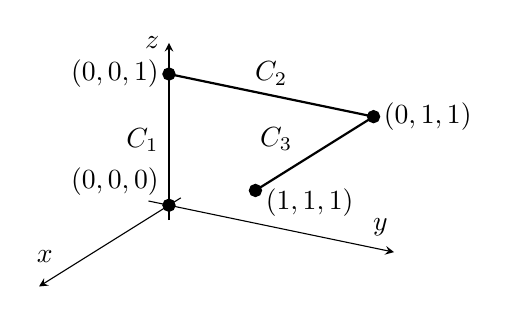
\begin{tikzpicture}[]
\begin{axis}[clip=false,small,view/h=120,axis lines=middle,xlabel={$x$},ylabel={$y$},zlabel={$z$},xtick={\empty},ytick={\empty},ztick={\empty},enlargelimits=true,zlabel style={anchor=east},zmax=1.125]
\addplot3[thick,mark=*]plot coordinates {(0,0,0)(0,0,1)}node[pos=0.5,left]{$C_1$}node[pos=0,above left]{$(0,0,0)$}node[pos=1,left]{$(0,0,1)$};
\addplot3[thick]plot coordinates {(0,0,1)(0,1,1)}node[pos=0.5,above]{$C_2$}node[right]{$(0,1,1)$};
\addplot3[thick,mark=*]plot coordinates {(0,1,1)(1,1,1)}node[pos=0.6,above left]{$C_3$}node[right,yshift=-1ex]{$(1,1,1)$};
\end{axis}
\end{tikzpicture}
\caption{ٹکڑوں میں خطی راہ برائے سوال \حوالہ{سوال_سمتی_تکمل_ٹکڑوں_خطی_راہ}}
\label{شکل_سوال_سمتی_تکمل_ٹکڑوں_خطی_راہ}
\end{minipage}
\end{figure}
\ابتدا{سوال}\شناخت{سوال_سمتی_تکمل_دائری_راہ}
تفاعل \عددی{f(x,y,z)=x+\sqrt{y}-z^2} کا تکمل \عددی{(0,0,0)} تا \عددی{(1,1,1)} درج ذیل راہ پر  چلتے ہوئے  تلاش کریں  (شکل \حوالہ{شکل_سوال_سمتی_تکمل_دائری_راہ})۔
\begin{align*}
C_1:\quad \kvec{r}(t)&=t\ai+t^2\aj,\quad 0\le t\le 1\\
C_2:\quad \kvec{r}(t)&=\ai+\aj+t\ak,\quad 0\le t\le 1
\end{align*}
\انتہا{سوال}
\ابتدا{جواب}
\wf{\unexpanded{\(\tfrac{1}{6}(5\sqrt{5}+9)\)}}
\انتہا{جواب}
%
\ابتدا{سوال}\شناخت{سوال_سمتی_تکمل_ٹکڑوں_خطی_راہ}
تفاعل \عددی{f(x,y,z)=x+\sqrt{y}-z^2} کا تکمل \عددی{(0,0,0)} تا \عددی{(1,1,1)} درج ذیل راہ پر  چلتے ہوئے  تلاش کریں  (شکل \حوالہ{شکل_سوال_سمتی_تکمل_ٹکڑوں_خطی_راہ})۔
\begin{align*}
C_1:\quad \kvec{r}(t)&=t\ak,\quad 0\le t\le 1\\
C_2:\quad \kvec{r}(t)&=t\aj+\ak,\quad 0\le t\le 1\\
C_3:\quad \kvec{r}(t)&=t\ai+\aj+\ak,\quad 0\le t\le 1
\end{align*}

\انتہا{سوال}
%
\ابتدا{سوال}
تفاعل \عددی{f(x,y,z)=\tfrac{x+y+z}{x^2+y^2+z^2}} کا تکمل راہ \عددی{\kvec{r}(t)=t\ai+t\aj+t\ak,\, 0<a\le t\le b} پر تلاش کریں۔
\انتہا{سوال}
\ابتدا{جواب}
\wf{\unexpanded{\(\sqrt{3}\ln\tfrac{b}{a}\)}}
\انتہا{جواب}
%
\ابتدا{سوال}
تفاعل \عددی{f(x,y,z)=-\sqrt{x^2+z^2}} کا تکمل درج ذیل دائری راہ پر تلاش کریں۔
\[\kvec{r}(t)=(a\cos t)\ai+(a\sin t)\ak,\quad 0\le t\le 2\pi\]
\انتہا{سوال}
%
\موٹا{مسطح منحنیات پر لکیری تکملات}\\
سوال \حوالہ{سوال_سمتی_تکمل_دی_گئی_منحنی-الف} تا سوال \حوالہ{سوال_سمتی_تکمل_دی_گئی_منحنی-ب} میں \عددی{f} کا تکمل دی گئی منحنی پر تلاش کریں۔

\ابتدا{سوال}\شناخت{سوال_سمتی_تکمل_دی_گئی_منحنی-الف}
\(f(x,y)=\frac{x^3}{y},\quad C:\, y=\frac{x^2}{2},\quad 0\le x\le 2\)
\انتہا{سوال}
\ابتدا{جواب}
\wf{\unexpanded{\(\tfrac{10\sqrt{5}-2}{3}\)}}
\انتہا{جواب}
%
\ابتدا{سوال}
\(f(x,y)=\frac{x+y^2}{\sqrt{1+x^2}},\quad C:\, y=\frac{x^2}{2},\quad \text{\RL{ \عددی{(1,\frac{1}{2})} سے \عددی{(0,0)} تک}}\)
\انتہا{سوال}
%
\ابتدا{سوال}
\(f(x,y)=x+y,\quad C:\, x^2+y^2=4,\quad \text{\RL{  ربع اول میں \عددی{(2,0)} سے \عددی{(0,2)} تک}}\)
\انتہا{سوال}
\ابتدا{جواب}
\wf{\unexpanded{\(8\)}}
\انتہا{جواب}
%
\ابتدا{سوال}\شناخت{سوال_سمتی_تکمل_دی_گئی_منحنی-ب}
\(f(x,y)=x^2-y,\quad C:\, x^2+y^2=4,\quad \text{\RL{  ربع اول میں \عددی{(0,2)} سے \عددی{(\sqrt{2},\sqrt{2})} تک}}\)
\انتہا{سوال}

\موٹا{کمیت اور معیار اثر}\\
%
\ابتدا{سوال}
ایک پتلی تار جس کی کثافت \عددی{\delta=\tfrac{3}{2}t} ہے منحنی \عددی{\kvec{r}(t)=(t^2-1)\aj+2t\ak,\, 0\le t\le 1} کے ساتھ ساتھ پائی جاتی ہے۔اس تار کی کمیت تلاش کریں۔
\انتہا{سوال}
\ابتدا{جواب}
\wf{\unexpanded{\(2\sqrt{2}-1\)}}
\انتہا{جواب}
%
\ابتدا{سوال}
ایک پتلی  تار جس کی کثافت \عددی{\delta(x,y,z)=15\sqrt{y+2}} ہے منحنی \عددی{\kvec{r}(t)=(t^2-1)\aj+2t\ak,\, -1\le t\le 1} کے ساتھ ساتھ پائی جاتی ہے۔اس تار کا مرکز کمیت تلاش کریں۔ اس منحنی کو ترسیم کر کے اس پر مرکز کمیت دکھائیں۔
\انتہا{سوال}
%
\ابتدا{سوال}
منحنی \عددی{\kvec{r}(t)=\sqrt{2}t\aj+(4-t^2)\ak\, 0\le t\le 1} کے ساتھ ساتھ  ایک پتلی تار پائی جانے والی تار کی کثافت (ا) \عددی{\delta=3t}، (ب) \عددی{\delta=1} ہے۔اس تار کا مرکز کمیت تلاش کریں۔
\انتہا{سوال}
\ابتدا{جواب}
\wf{\unexpanded{
(ا) \عددی{4\sqrt{2}-1}، (ب) \عددی{\sqrt{2}+\ln(1+\sqrt{2})}
}}
\انتہا{جواب}
%
\ابتدا{سوال}
ایک پتلی تار جس کی کثافت \عددی{\delta=3\sqrt{5+t}} ہے منحنی
 \عددی{\kvec{r}(t)=t\ai+2t\aj+\tfrac{2}{3}t^{3/2}\ak,\, 0\le t\le 2} کے ساتھ ساتھ پائی جاتی ہے۔ اس تار کی کمیت تلاش کریں۔
\انتہا{سوال}
%
\ابتدا{سوال}
مستوی \عددی{xy} میں دائرہ \عددی{x^2+y^2=a^2} پر مستقل کثافت \عددی{\delta} کی ایک پتلی تار پائی جاتی ہے۔ محور \عددی{z} کے لحاظ سے اس تار کا جمودی معیار اثر اور رداس  دوار تلاش کریں۔
\انتہا{سوال}
\ابتدا{جواب}
\wf{\unexpanded{
\عددی{I_z=2\pi\delta a^3}، \عددی{R_z=a}
}}
\انتہا{جواب}
%
\ابتدا{سوال}
مستوی \عددی{yz} میں لکیری قطع \عددی{\kvec{r}(t)=t\aj+(2-2t)\ak,\, 0\le t\le 1} پر مستقل کثافت  کی ایک پتلی تار پائی جاتی ہے۔ تینوں محددی محوروں  کے لحاظ سے اس تار کا جمودی معیار اثر اور رداس  دوار تلاش کریں۔
\انتہا{سوال}
%
\ابتدا{سوال}
مستقل کثافت \عددی{\delta} کی ایک پتلی تار پیچدار منحنی \عددی{\kvec{r}(t)=(\cos t)\ai+(\sin t)\aj+t\ak,\, 0\le t\le 2\pi} کے ساتھ ساتھ پائی جاتی ہے۔ (ا) \عددی{I_z} اور \عددی{R_z} تلاش کریں۔ (ب) فرض کریں مستقل کثافت \عددی{\delta} کی ایک دوسری پتلی تار، جس کی لمبائی دگنی ہے (\عددی{0\le t\le 4\pi})، اسی منحنی \عددی{\kvec{r}(t)} کے ساتھ ساتھ پائی جاتی ہے۔ بغیر حل کیے بتلائیں کہ آیا اس تار کا جمودی معیار اثر اور رداس دوار پہلی تار سے مختلف ہوں گے؟  اب انہیں حل کر کے اپنے جواب کی تصدیق کریں۔
\انتہا{سوال}
\ابتدا{جواب}
\wf{\unexpanded{
(ا) \عددی{I_z=2\pi\sqrt{2}\delta}، \عددی{R_z=1}؛\\ (ب) \عددی{I_z=4\pi\sqrt{2}\delta}، \عددی{R_z=1}
}}
\انتہا{جواب}
%
\ابتدا{سوال}
منحنی \عددی{\kvec{r}(t)=(t\cos t)\ai+(t\sin t)\aj+(\tfrac{2\sqrt{2}}{3})t^{3/2}\ak,\, 0\le t\le 1} کے ساتھ ساتھ مستقل کثافت \عددی{\delta =1} کی ایک پتلی تار  پائی جاتی ہے۔ اس کی \عددی{\overline{z}}، \عددی{I_z} اور \عددی{R_z} تلاش کریں۔
\انتہا{سوال}
%
\ابتدا{سوال}
\عددی{I_z} اور \عددی{R_z} مثال \حوالہ{مثال_سمتی_تکمل_قوس_کی_کمیت} کی محراب کے لئے تلاش کریں۔
\انتہا{سوال}
\ابتدا{جواب}
\wf{\unexpanded{
\عددی{I_z=2\pi-2}، \عددی{R_z=1}
}}
\انتہا{جواب}
%
\ابتدا{سوال}
ایک پتلی تار جس کی کثافت \عددی{\delta=\tfrac{1}{t+1}} ہے منحنی \عددی{\kvec{r}(t)=t\ai+\tfrac{2\sqrt{2}}{3}t^{3/2}\aj+\tfrac{t^2}{2}\ak,\, 0\le t\le 2} کے ساتھ ساتھ پائی جاتی ہے۔ اس تار کا مرکز کمیت اور محددی محوروں کے لحاظ سے جمودی معیار اثر اور رداس دوار تلاش کریں۔
\انتہا{سوال}
\موٹا{کمپیوٹر کا استعمال}\\
سوال \حوالہ{سوال_سمتی_تکمل_کمپیوٹر_الف} تا سوال \حوالہ{سوال_سمتی_تکمل_کمپیوٹر_ب} میں کمپیوٹر پر درج ذیل اقدام سے تکمل کی قیمت تلاش کریں۔
\begin{enumerate}[a.]
\item
راہ \عددی{\kvec{r}(t)=g(t)\ai+h(t)\aj+k(t)\ak} کے لئے \عددی{\dif s=\abs{\kvec{v}(t)}\dif t} دریافت کریں۔
\item
متکمل \عددی{f(g(t),h(t),k(t))\abs{\kvec{v}(t)}} کو مقدار معلوم \عددی{t} کا تفاعل لکھیں۔
\item
تکمل \عددی{\int_C f\dif s} کی قیمت مساوات \حوالہ{مساوات_میدان_خطی_تکمل_پ} کی مدد سے حاصل  کریں۔ 
\end{enumerate}
%
\ابتدا{سوال}\شناخت{سوال_سمتی_تکمل_کمپیوٹر_الف}
\(f(x,y,z)=\sqrt{1+30x^2+10y};\quad \kvec{r}(t)=t\ai+t^2\aj+3t^2\ak,\quad 0\le t\le 2\)
\انتہا{سوال}
%
\ابتدا{سوال}
\(f(x,y,z)=\sqrt{1+x^3+5y^3};\quad \kvec{r}(t)=t\ai+\frac{1}{3}t^2\aj+\sqrt{t}\ak,\quad 0\le t\le 2\)
\انتہا{سوال}
%
\ابتدا{سوال}
\(f(x,y,z)=x\sqrt{y}-3z^2;\,\kvec{r}(t)=\cos 2t \ai+\sin 2t\aj+5t\ak,\quad 0\le t\le 2\pi\)
\انتہا{سوال}
%
\ابتدا{سوال}\شناخت{سوال_سمتی_تکمل_کمپیوٹر_ب}
\(f(x,y,z)=\big(1+\frac{9}{4}z^{1/3}\big)^{1/4};\, \kvec{r}(t)=\kvec{r}(t)=\cos 2t \ai+\sin 2t\aj+t^{5/2}\ak,\)\\
\( 0\le t\le 2\pi\quad\quad\quad\quad\quad\quad\)
\انتہا{سوال}
\انتہا{سوالات}
%%%%%%%%%%%%%%%%%%%%%%%%%
\حصہ{سمتی میدان، کام، دائری بہاو، اور بہاو}
ان طبیعی  مظہر  کے مطالعہ کے دوران، جنہیں سمتیات سے ظاہر کیا جاتا ہے، بند راہ پر تکملات کی بجائے سمتی میدان میں راہ پر تکملات استعمال کیے جاتے ہیں۔متغیر قوت کے خلاف ایک مقام سے دوسری مقام کسی جسم کو منتقل کرنے (جیسا قوت ثقل کے خلاف خلاء میں سواری بھیجنے)   یا سمتی میدان میں ایک جسم کو کسی راہ پر حرکت دینے (جیسا مسرع کسی ذرے کی توانائی بڑھاتا ہو)  کے لئے درکار کام   اس طرح کے تکملات سے حاصل کیے  جاتے ہیں۔  منحنیات عبور کرتا ہوا سیال کے بہاو کی شرح بھی لکیری تکملات سے حاصل کی جاتی ہے۔

\جزوحصہء{سمتی میدان}
مستوی یا فضا میں دائرہ کار پر  \اصطلاح{سمتی میدان}\فرہنگ{میدان!سمتی}\حاشیہب{vector field}\فرہنگ{field!vector} سے مراد ایسا تفاعل ہے جو دائرہ کار کے ہر نقطہ کو ایک سمتیہ مختص کرتا ہو۔سہ ابعادی سمتیات کے میدان کا ایک کلیہ درج ذیل ہو سکتا ہے۔
\begin{align*}
\kvec{F}(x,y,z)=M(x,y,z)\ai+N(x,y,z)\aj+P(x,y,z)\ak
\end{align*}
استمراری جزوی تفاعل \عددی{M}، \عددی{N}، \عددی{P} کی صورت میں یہ میدان استمراری ہو گا، قابل تفرق \عددی{M}، \عددی{N}، \عددی{P} کی صورت میں یہ میدان قابل تفرق ہو گا، وغیرہ وغیرہ۔ دو ابعادی سمتیات کے میدان کا ایک کلیہ درج ذیل ہو سکتا ہے۔
\begin{align*}
\kvec{F}(x,y)=M(x,y)\ai+N(x,y)\aj
\end{align*}
گول انداز کی گزرگاہ کے مستوی میں  گزرگاہ کے ہر نقطہ کے ساتھ گول انداز کا سمتی رفتاری سمتیہ منسلک کرنے سے گزرگاہ  کی ہمراہ دو ابعادی میدان حاصل ہو گا۔  غیر سمتی تفاعل کے ہم قد سطح کے ہر نقطہ کے ساتھ  تفاعل کا سمتیہ ڈھلوان منسلک کرنے سے سطح پر سہ ابعادی میدان حاصل ہو گا۔   متحرک سیال کے ہر نقطہ کے ساتھ سمتی رفتاری سمتیہ منسلک کرنے سے فضا میں اس خطہ پر سہ ابعادی  میدان حاصل ہو گا۔ بشمول ان  کے چند  میدان  شکل میں دکھائے گئے ہیں جہاں کچھ میدانوں کے کلیات بھی دیے گئے ہیں۔
 

وہ میدان ترسیم کرنے کے لئے جن کے کلیات معلوم ہوں، ہم دائرہ کار میں چند نقطے منتخب کر کے ان نقطوں پر نقطوں کے ساتھ منسلک سمتیات  کا خاکہ بناتے ہیں۔ دھیان رہے کہ روایتی طور پر اس نقطہ پر، جہاں سمتی تفاعل کی قیمت حاصل کی گئی ہو،  سمتیہ ظاہر کرنے والی تیر دار لکیر  کی دم  رکھی جاتی ہے نا کہ سر۔ تعین گر سمتیات (باب \حوالہ{سمتی_قیمت_تفاعل_اور_فضا_میں_حرکت}) کے لئے ایسا نہیں کیا جاتا ہے بلکہ تعین گر سمتیات کو ظاہر کرنے والی تیر دار لکیر کی دم کو مبدا پر رکھا جاتا ہے جبکہ اس کا سر  سیارہ یا گول انداز کے مقام پر رکھا جاتا ہے۔

\جزوحصہء{میدان ڈھلوان}
\ابتدا{تعریف}
قابل تفرق تفاعل \عددی{f(x,y,z)} کے \اصطلاح{میدان ڈھلوان}\فرہنگ{میدان!ڈھلوان}\حاشیہب{gradient field}\فرہنگ{gradient!field} سے مراد سمتیات ڈھلوان
\begin{align*}
\nabla f=\frac{\partial f}{\partial x}\ai+\frac{\partial f}{\partial y}\aj+\frac{\partial f}{\partial z}\ak
\end{align*}
 کا میدان ہے۔
\انتہا{تعریف}
%=======================
\ابتدا{مثال}
تفاعل \عددی{f(x,y,z)=xyz} کا میدان ڈھلوان تلاش کریں۔

حل:\quad
تفاعل \عددی{f} کے میدان ڈھلوان سے مراد میدان \عددی{\kvec{F}=\nabla f=yz\ai+xz\aj+xy\ak} ہے۔
\انتہا{مثال}
%=====================

 ہم  دیکھیں گے کہ انجینئری، ریاضیات، طبیعیات، وغیرہ میں میدان ڈھلوان  خصوصی اہمیت رکھتے ہیں۔

\جزوحصہء{فضا میں منحنی کی ہمراہ قوت کا کیا ہوا کام}
فرض کریں  فضا کے ایک خطہ  میں سمتی میدان \عددی{\kvec{F}=M(x,y,z)\ai+N(x,y,z)\aj+P(x,y,z)\ak}  ایک قوت کو ظاہر کرتا ہے (یہ قوت ثقل  یا کسی قسم کی برقناطیسی قوت ہو سکتی ہے) جبکہ اس خطہ میں درج ذیل ایک ہموار منحنی ہے۔
\begin{align*}
\kvec{r}(t)=g(t)\ai+h(t)\aj+k(t)\ak,\quad a\le t\le b
\end{align*}
ایسی صورت میں منحنی پر \عددی{\kvec{F}\cdot\kvec{T}}،  اکائی مماسی سمتیہ کے رخ \عددی{\kvec{F}} کا غیر سمتی جزو، کے تکمل کو \عددی{a} تا \عددی{b} \عددی{\kvec{F}} کا کیا ہوا کام کہتے ہیں۔

\ابتدا{تعریف}
ہموار منحنی \عددی{\kvec{r}(t)=g(t)\ai+h(t)\aj+k(t)\ak} پر \عددی{a} تا \عددی{b} قوت
 \عددی{\kvec{F}=M(x,y,z)\ai+N(x,y,z)\aj+P(x,y,z)\ak} کا کیا ہوا کام \عددی{W} درج ذیل ہو گا۔
\begin{align}\label{مساوات_سمتی_میدان_کام_کی_تعریف}
W=\int_{t=1}^{t=b}\kvec{F}\cdot \kvec{T}\dif s
\end{align}
\انتہا{تعریف}
%=======================

 مثبت محور \عددی{x} رخ  مقدار \عددی{F(x)} کی استمراری قوت کے کام کا کلیہ  \عددی{W=\int_a^bF(x)\dif x} حصہ \حوالہ{حصہ_تکمل_استعمال_کام} میں اخذ کیا گیا۔مساوات \حوالہ{مساوات_سمتی_میدان_کام_کی_تعریف} کے حصول کے دلائل وہی ہیں۔ ہم منحنی کو چھوٹے قطعات میں تقسیم کر کے، ہر قطع پر کام کو تخمیناً مستقل قوت ضرب فاصلہ لے کر،  نتائج کے مجموعہ کو منحنی پر کام کی تخمینی قیمت حاصل کرتے ہیں، اور قطعات کی تعداد زیادہ سے زیادہ کر کے ہر قطع کی لمبائی کم سے کم کرتے ہوئے، تخمینی مجموعات کی تحدیدی قیمت کو کام کی تعریف لیتے ہیں۔ یہ جاننے کے لئے کہ تحدیدی تکمل کی قیمت کیا ہو گی، ہم قطع \عددی{ِ=[a,b]} کی خانہ بندی عمومی طرح  کر کے ہر ذیلی قطع \عددی{[t_k,t_{k+1}]} پر نقطہ \عددی{c_k} منتخب کرتے ہیں۔ قطع \عددی{I} کی خانہ بندی  منحنی کی خانہ بندی تعین (پیدا) کرتی ہے، جہاں تعین گر سمتیہ \عددی{\kvec{r}} کا سر نقطہ \عددی{N_k} پر ہو گا اور ذیلی قطع \عددی{N_kN_{k+1}} کی لمبائی \عددی{\Delta s_k} ہو گی۔ اگر منحنی پر \عددی{t=c_k} کے مطابقتی نقطہ  پر \عددی{\kvec{F}} کی قیمت \عددی{\kvec{F}_k} اور منحنی کا مماسی سمتیہ \عددی{\kvec{T}_k} ہو تب \عددی{t=c_k}  پر \عددی{\kvec{T}} کے رخ \عددی{\kvec{F}} کا غیر سمتی جزو \عددی{\kvec{F}_k\cdot\kvec{T}_k} ہو گا۔ منحنی کے قطع \عددی{N_kN_{k+1}} کی ہمراہ \عددی{\kvec{F}} کا کیا ہوا کام تخمیناً درج ذیل ہو گا۔
\begin{align*}
(\text{\RL{حرکت کے رخ قوت کا جزو}})\times (\text{\RL{طے فاصلہ}})=\kvec{F}_k\cdot\kvec{T}_k\Delta s_k
\end{align*}
منحنی کی ہمراہ  \عددی{t=a} تا \عددی{t=b} کام تخمیناً درج ذیل ہو گا۔
\begin{align*}
\sum_{k=1}^{n}\kvec{F}_k\cdot\kvec{T}_k\Delta s_k
\end{align*}
جیسا جیسا \عددی{[a,b]} کے خانہ بندی کا معیار صفر کے قریب سے قریب ہوتا  ہے، ویسے ویسے منحنی کی پیدا کردہ خانہ بندی کا معیار بھی صفر کے قریب سے قریب ہوتا ہے اور مجموعہ درج ذیل لکیری تکمل کو پہنچتا ہے۔
\begin{align*}
\int_{t=a}^{t=b}\kvec{F}\cdot\kvec{T}\dif s
\end{align*} 
اس تکمل سے حاصل عدد کی علامت، \عددی{t} بڑھانے سے حاصل  پر چلنے کے، رخ پر منحصر ہو گی۔ منحنی پر چلنے کا رخ الٹ کرنے سے \عددی{\kvec{T}} کا رخ الٹ ہو گا جس کی بنا \عددی{\kvec{F}\cdot\kvec{T}} اور تکمل کی علامت الٹ ہو گی۔ 

\جزوحصہء{علامتیت اور قیمت کا حصول}
تکمل کام (مساوات \حوالہ{مساوات_سمتی_میدان_کام_کی_تعریف}) کو لکھنے کے چھ طریقے درج ذیل ہیں۔
\begin{gather}
\begin{aligned}\label{مساوات_سمتی_تکمل_متعدد_روپ_کام}
W&=\int_{t=a}^{t=b}\kvec{F}\cdot\kvec{T}\dif s&&\text{\RL{تعریف}}\\
&=\int_{t=a}^{t=b}\kvec{F}\cdot\dif \kvec{r}&&\text{\RL{مختصر تفریقی روپ}}\\
&=\int_{t=a}^{t=b}\kvec{F}\cdot\frac{\dif \kvec{r}}{\dif t}\dif t&&
\text{\RL{پھیلا کر \عددی{\dif t}  شامل کیا گیا ہے}}\\
&=\int_{t=a}^{t=b}\big(M\frac{\dif g}{\dif t}+N\frac{\dif h}{\dif t}+P\frac{\dif k}{\dif t}\big)\dif t&&\text{\RL{مقدار معلوم \عددی{t} اور سمتی رفتار \عددی{\frac{\dif\kvec{r}}{\dif t}} اجاگر کیے گئے}}\\
&=\int_{t=a}^{t=b}\big(M\frac{\dif x}{\dif t}+N\frac{\dif y}{\dif t}+P\frac{\dif z}{\dif t}\big)\dif t&&\text{\RL{جزوی تفاعل اجاگر کیے گئے}}\\
&=\int_{t=a}^{t=b} M\dif x+N\dif y+P\dif z&&\text{\RL{\عددی{\dif t} منسوخ کر کے عمومی روپ حاصل کی گئی}}
\end{aligned}
\end{gather}

مساوات \حوالہ{مساوات_سمتی_تکمل_متعدد_روپ_کام} کے کلیات کی  قیمتوں کا حصول،  بظاہر مختلف روپ  کے باوجود،  ایک ہی طرح کیا جاتا ہے۔ 

\موٹا{تکمل کام کی قیمت کا حصول}\\
تکمل کام کی قیمت حاصل کرنے کے اقدام درج ذیل ہیں۔
\begin{enumerate}[1.]
\item
منحنی پر \عددی{\kvec{F}} کی قیمت مقدار معلوم \عددی{t} کے تفاعل کی روپ میں لکھیں۔
\item
تفرق \عددی{\frac{\dif \kvec{r}}{\dif t}} تلاش کریں۔
\item
\عددی{\kvec{F}} اور \عددی{\frac{\dif\kvec{r}}{\dif t}} کا غیر سمتی ضرب لیں۔
\item
\عددی{t=a} سے \عددی{t=b} تک تکمل کریں۔
\end{enumerate}

%==================
\ابتدا{مثال}
منحنی \عددی{\kvec{r}(t)=t\ai+t^2\aj+t^3\ak,\,0\le t\le 1} کی ہمراہ  \عددی{(0,0,0)} سے  \عددی{(1,1,1)}  تک \عددی{\kvec{F}=(y-x^2)\ai+(z-y^2)\aj+(x-z^2)\ak} کا کام  تلاش کریں۔

حل:\\
پہلا قدم:\quad
منحنی پر \عددی{\kvec{F}} کی قیمت کا حصول۔
\begin{align*}
\kvec{F}&=(y-x^2)\ai+(z-y^2)\aj+(x-z^2)\ak\\
&=(\underbrace{t^2-t^2}_0)\ai+(t^3-t^4)\aj+(t-t^6)\ak
\end{align*}
دوسرا قدم:\quad
\عددی{\frac{\dif \kvec{r}}{\dif t}} حاصل کرتے ہیں۔
\begin{align*}
\frac{\dif \kvec{r}}{\dif t}&=\frac{\dif}{\dif t}(t\ai+t^2\aj+t^3\ak)=\ai+2t\aj+3t^2\ak
\end{align*}
تیسرا قدم:\quad
\عددی{\kvec{F}} اور \عددی{\frac{\dif\kvec{r}}{\dif t}} کا غیر سمتی ضرب۔
\begin{align*}
\kvec{F}\cdot\frac{\dif\kvec{r}}{\dif t}&=[(t^3-t^4)\aj+(t-t^6)\ak]\cdot(\ai+2t\aj+3t^2\ak)\\
&=(t^3-t^4)(2t)+(t-t^6)(3t^2)=2t^4-2t^5+3t^3-3t^8
\end{align*}
چوتھا قدم:\quad
\عددی{t=0} تا \عددی{t=1} تکمل۔
\begin{align*}
\text{کام}=W&=\int_0^1(2t^4-2t^5+3t^3-3t^8)\dif t\\
&=\big[\frac{2}{5}t^5-\frac{2}{6}t^6+\frac{3}{4}t^4-\frac{3}{9}t^9\big]_0^1=\frac{29}{60}
\end{align*}
\انتہا{مثال}
%============

\جزوحصہء{تکمل ہمراہ بہاو اور دائری بہاو}
فرض کریں \عددی{\kvec{F}=M\ai+N\aj+P\ak} میدان قوت کی بجائے  فضا کے ایک خطہ (مثلاً پانی سے چلنے والے جنریٹر کا چرخی خانہ   یا سمندری طاس) میں بہتا ہوا سیال کے سمتی رفتاری میدان  کو ظاہر کرتا ہے ۔ ایسی صورت میں منحنی کی ہمراہ 
 \عددی{\kvec{F}\cdot \kvec{T}} کا تکمل، منحنی کی ہمراہ سیال کا بہاو دے گا۔

\ابتدا{تعریف}
استمراری سمتی رفتاری میدان کے دائرہ کار میں ہموار منحنی \عددی{\kvec{r}(t)=g(t)\ai+h(t)\aj+k(t)\ak,\, a\le t\le b} پر \عددی{a} سے \عددی{b} تک \عددی{\kvec{F}\cdot\kvec{T}} کا تکمل،    \عددی{t=a} سے \عددی{t=b} تک  منحنی کا  ہمراہ بہاو دے گا:
\begin{align}
\text{\RL{ہمراہ بہاو}}=\int_a^b \kvec{F}\cdot\kvec{T}\dif s
\end{align}
اس تکمل کو \اصطلاح{تکمل ہمراہ بہاو}\فرہنگ{تکمل!ہمراہ بہاو}\حاشیہب{flow integral}\فرہنگ{flow!integral} کہتے ہیں۔ بند منحنی کی صورت میں اس بہاو کو  منحنی کے گرد منحنی کی ہمراہ \اصطلاح{دائری بہاو}\فرہنگ{دائری بہاو}\حاشیہب{circulation}\فرہنگ{circulation} کہتے ہیں۔
\انتہا{تعریف}
%========================

تکمل ہمراہ بہاو کی قیمت  بھی تکمل کام کی قیمت کی طرح حاصل کی جاتی ہے۔

\ابتدا{مثال}
ایک سیال کا  سمتی رفتاری میدان \عددی{\kvec{F}=x\ai+z\aj+y\ak} ہے۔ درج ذیل پیچدار منحنی کے ساتھ ساتھ اس کی ہمراہ بہاو تلاش کریں۔
\[\kvec{r}(t)=(\cos t)\ai+(\sin t)\aj+t\ak,\, 0\le t\le \tfrac{\pi}{2}\]

حل:\\
پہلا قدم:\quad
منحنی پر \عددی{\kvec{F}} کی قیمت تلاش کرتے ہیں۔
\begin{align*}
\kvec{F}=x\ai+z\aj+y\ak=(\cos t)\ai+(\sin t)\ai+t\ak
\end{align*}
دوسرا قدم:\quad
\عددی{\tfrac{\dif \kvec{r}}{\dif t}} تلاش کرتے ہیں۔
\begin{align*}
\frac{\dif \kvec{r}}{\dif t}=(-\sin t)\ai+(\cos t)\aj+\ak
\end{align*}
تیسرا قدم:\quad
غیر سمتی ضرب \عددی{\kvec{F}\cdot \tfrac{\dif\kvec{r}}{\dif t}} تلاش کرتے ہیں۔
\begin{align*}
\kvec{F}\cdot\frac{\dif \kvec{r}}{\dif t}&=(\cos t)(-\sin t)+(t)(\cos t)+(\sin t)(1)\\
&=-\sin t\cos t+t\cos t+\sin t
\end{align*}
چوتھا قدم:\quad
\عددی{t=a} تا \عددی{t-b} تکمل لیتے ہیں۔
\begin{align*}
\text{بہاو}&=\int_{t=a}^{t=b} \kvec{F}\cdot \frac{\dif \kvec{r}}{\dif t}\dif t=\int_0^{\pi/2}(-\sin t\cos t+t\cos t+\sin t)\dif t\\
&=\big[\frac{\cos^2t}{2} +\sin t\big]_0^{\pi/2}=\big(0+\frac{\pi}{2}\big)-\big(\frac{1}{2}+0\big)=\frac{\pi}{2}-\frac{1}{2}
\end{align*}
\انتہا{مثال}
%==================== 
\ابتدا{مثال}
میدان \عددی{\kvec{F}=(x-y)\ai+x\aj} کا دائرہ \عددی{\kvec{r}(t)=(\cos t)\ai+(\sin t)\aj,\, 0\le t\le 2\pi} کی ہمراہ دائرہ کے گرد دائری بہاو تلاش کریں۔

حل:\quad
\begin{enumerate}[1.]
\item
دائرہ پر \عددی{\kvec{F}=(x-y)\ai+x\aj=(\cos t-\sin t)\ai+(\cos t)\aj} ہو گا۔
\item
\(\frac{\dif \kvec{r}}{\dif t}=(-\sin t)\ai+(\cos t)\aj\)
\item
\(\kvec{F}\cdot \frac{\dif \kvec{r}}{\dif t}=-\sin t\cos t+\underbrace{\sin^2t+\cos^2t}_1\)
\item
دائری بہاو درج ذیل ہو گا۔
\begin{align*}
\text{\RL{دائری بہاو}}&=\int_0^{2\pi}\kvec{F}\cdot \frac{\dif \kvec{r}}{\dif t}\dif t=\int_0^{2\pi}(1-\sin t\cos t)\dif t\\
&=\big[t-\frac{\sin^2t}{2}\big]_0^{2\pi}=2\pi
\end{align*}
\end{enumerate}
\انتہا{مثال}
%==================

\جزوحصہء{مستوی منحنی کو عبور کرتا ہوا  بہاو}
مستوی \عددی{xy} میں ہموار بند منحنی \عددی{C} میں محیط خطہ سے سیال کے اخراج و دخول کی شرح  \عددی{C} پر  \عددی{\kvec{F}\cdot\kvec{n}} ( منحنی کے بیرونی  عمودی اکائی سمتیہ  کے رخ رفتاری میدان کے غیر سمتی جزو)  کے لکیری تکمل سے حاصل ہو گی۔ اس تکمل کی قیمت کو  \عددی{C} عبور کرتا ہوا \عددی{\kvec{F}} کا بہاو (یا \اصطلاح{نفاذ}\فرہنگ{نفاذ}) کہتے ہیں۔ برقی یا مقناطیسی میدان \عددی{\kvec{F}} کی صورت میں بھی اس تکمل کی قیمت کو \عددی{C} عبور کرتا ہوا بہاو یا نفاذ کہیں گے اگرچہ ان میں کوئی بہتا ہوا سیال نہیں پایا جاتا ہے۔

\ابتدا{تعریف}
استمراری سمتی میدان \عددی{\kvec{F}=M(x,y)\ai+N(x,y)\aj} کے دائرہ کار میں ہموار مسطح بند منحنی \عددی{C} جس کا بیرونی رخ عمودی اکائی سمتیہ \عددی{\kvec{n}} ہو کی صورت میں \عددی{C} کو عبور کرتا ہوا \عددی{\kvec{F}} کا \اصطلاح{بہاو}\فرہنگ{بہاو}\حاشیہب{flux}\فرہنگ{flux} درج ذیل تکمل دے گا۔
\begin{align}\label{مساوات_سمتی_تکمل_عبور_کرتا_بہاو_تعریف}
\text{\RL{\(C\) عبور کرتا ہوا \(\kvec{F}\) کا بہاو}}=\int_C \kvec{F}\cdot \kvec{n}\dif s
\end{align}
\انتہا{تعریف}

منحنی کو عبور کرتے ہوئے بہاو (نفاذ) اور دائری بہاو میں فرق سے واقف ہونا ضروری ہے۔ منحنی \عددی{C} کو عبور کرتا ہوا \عددی{\kvec{F}} کے بہاو سے مراد منحنی  پر \عددی{\kvec{F}\cdot\kvec{n}} (منحنی کے بیرونی عمود کے رخ \عددی{\kvec{F}} کے غیر سمتی جزو) کا تکمل ہے۔ بند منحنی \عددی{C} کے گرد \عددی{\kvec{F}} کے دائری بہاو سے مراد منحنی پر \عددی{\kvec{F}\cdot\kvec{T}} (منحنی کے اکائی مماس کے رخ \عددی{\kvec{F}} کے غیر سمتی جزو) کا تکمل ہے۔ منحنی عبور کرتا ہوا بہاو سے مراد \عددی{\kvec{F}} کے عمودی جزو کا تکمل جبکہ دائری بہاو سے مراد \عددی{\kvec{F}} کے مماسی جزو کا تکمل ہے۔ روز مرہ زندگی میں منحنی کو عبور کرتے ہوئے بہاو یعنی نفاذ کو مختصراً \اصطلاح{بہاو} کہا جاتا ہے۔

مساوات \حوالہ{مساوات_سمتی_تکمل_عبور_کرتا_بہاو_تعریف} کے تکمل کی قیمت معلوم کرنے کی خاطر ہم مقدار معلوم روپ 
\begin{align*}
x=g(t),\quad y=h(t),\quad a\le t\le b
\end{align*}
سے ابتدا کرتے ہیں۔یوں \عددی{t} کی قیمت \عددی{a} سے  \عددی{b} تک بڑھانے سے منحنی پر ایک سر سے دوسرے سر تک ٹھیک ایک بار چلا جائے گا۔ منحنی کے اکائی مماسی سمتیہ \عددی{\kvec{T}} اور کارتیسی محددی نظام کے اکائی سمتیہ \عددی{\kvec{k}} کا سمتی ضرب منحنی کا بیرونی اکائی عمودی سمتیہ \عددی{\kvec{n}} دے گا۔ سوال پیدا ہوتا ہے کہ ایسے دو سمتی ضرب \عددی{\kvec{T}\times\kvec{k}} اور \عددی{\kvec{k}\times\kvec{T}} پائے جاتے ہیں۔ان میں کونسا بیرونی اکائی سمتیہ دے گا؟ مقدار معلوم \عددی{t} بڑھانے سے \عددی{C} پر چلنے کے رخ پر اس کا جواب منحصر ہو گا۔ اگر منحنی پر حرکت گھڑی وار ہو تب \عددی{\kvec{k}\times\kvec{T}} بیرونی اکائی سمتیہ دے گا جبکہ خلاف گھڑی حرکت کی صورت میں \عددی{\kvec{T}\times\kvec{k}} بیرونی اکائی سمتیہ دے گا۔ عموماً خلاف گھڑی حرکت کے لئے کلیات اخذ کیے جاتے ہیں۔ یوں  \عددی{\kvec{n}=\kvec{T}\times\kvec{k}} ہو گا۔اگرچہ مساوات \حوالہ{مساوات_سمتی_تکمل_عبور_کرتا_بہاو_تعریف} میں دیے گئے تکمل کی قیمت منحنی پر چلنے کے رخ پر منحصر نہیں ہے، ہم خلاف گھڑی حرکت تصور کرتے ہوئے   مساوات \حوالہ{مساوات_سمتی_تکمل_عبور_کرتا_بہاو_تعریف} کو حل کرنے کے کلیات اخذ کرتے ہیں۔ 

ارکان کی صورت میں درج ذیل ہو گا۔
\begin{align*}
\kvec{n}=\kvec{T}\times\kvec{k}=\big(\frac{\dif x}{\dif s}\ai+\frac{\dif y}{\dif s}\aj\big)\times \kvec{k}=\frac{\dif y}{\dif s}\ai-\frac{\dif x}{\dif s}\aj
\end{align*}
اگر \عددی{\kvec{F}=M(x,y)\ai+N(x,y)\aj} ہو تب
\begin{align*}
\kvec{F}\cdot \kvec{n}=M(x,y)\frac{\dif y}{\dif s}-N(x,y)\frac{\dif x}{\dif s}
\end{align*}
لہٰذا
\begin{align*}
\int_C\kvec{F}\cdot\kvec{n}\dif s=\int_C\big(M\frac{\dif y}{\dif s}-N\frac{\dif x}{\dif s}\big)\dif s
\end{align*}
ہو گا جس سے درج ذیل حاصل ہوتا ہے۔
\begin{align}\label{مساوات_سمتی_تکمل_نفاذ}
\int_C\kvec{F}\cdot\kvec{n}\dif s=\oint_C M\dif y-N\dif x
\end{align}
 یاد رہے کہ \عددی{C} پر خلاف گھڑی چلتے ہوئے  بند تکمل \عددی{\oint} کی قیمت حاصل کی جائے گی۔ اس تکمل کے حصول کی خاطر ہم \عددی{M}، \عددی{\dif y}، \عددی{N} اور \عددی{\dif x} کو مقدار معلوم \عددی{t} کی روپ میں لکھ کر \عددی{t=a} تا \عددی{t=b} تکمل لیتے ہیں۔ہمیں بہاو (نفاذ) تلاش کرنے کے لئے  \عددی{\kvec{n}} یا \عددی{\dif s} جاننے کی ضرورت پیش نہیں آتی ہے۔ منحنی \عددی{C} پر خلاف گھڑی ٹھیک ایک بار چلتے ہوئے  کوئی بھی ہموار مقدار معلوم روپ \عددی{x=g(t)}، \عددی{y=h(t)}، جہاں \عددی{a\le t\le b} ہو، استعمال کیا جا سکتا ہے۔

\ابتدا{مثال}
مستوی \عددی{xy} میں دائرہ \عددی{x^2+y^2=1} کو پار کرتا ہوا \عددی{\kvec{F}=(x-y)\ai+x\aj} کا بہاو (نفاذ) تلاش کریں۔

حل:\quad
مقدار معلوم روپ \عددی{\kvec{r}(t)=(\cos t)\ai+(\sin t)\aj,\, 0\le t\le 2\pi} دائرے پر ٹھیک ایک بار چلتا ہے لہٰذا مساوات \حوالہ{مساوات_سمتی_تکمل_نفاذ} حل کرنے کی خاطر درج ذیل لیے جا سکتے ہیں۔
\begin{align*}
M&=x-y=\cos t-\sin t,&&\dif y=\dif\,(\sin t)=\cos t\dif t\\
N&=x=\cos t,&&\dif x=\dif\,(\cos t)=-\sin t\dif t
\end{align*}
یوں درج ذیل ہو گا۔
\begin{align*}
\text{\RL{}}&=\int_C M\dif y-N\dif x=\int_0^{2\pi}(\cos^2t-\sin t\cos t+\cos t\sin t)\dif t&& \text{\RL{مساوات \حوالہ{مساوات_سمتی_تکمل_نفاذ}}}\\
&=\int_0^{2\pi}\cos^2 t\dif t=\int_0^{2\pi}\frac{1+\cos 2t}{2}\dif t=\big[\frac{t}{2}+\frac{\sin 2t}{4}\big]_0^{2\pi}=\pi
\end{align*}
دائرہ کو عبور کرتا ہوا \عددی{\kvec{F}} کا بہاو \عددی{\pi} ہے۔چونکہ نتیجہ مثبت ہے لہٰذا دائرے سے کل بہاو کا رخ باہر کو ہو گا۔ دائرے میں دخول کی صورت میں نتیجہ منفی ہوتا۔
\انتہا{مثال}
%===========

\جزوحصہء{سوالات}
\ابتدا{سوالات}
\موٹا{سمتی میدان اور میدان ڈھلوان}\\
سوال \حوالہ{سوال_سمتی_تکمل_میدان_ڈھلوان_الف} تا سوال \حوالہ{سوال_سمتی_تکمل_میدان_ڈھلوان_ب} میں تفاعل کے میدان ڈھلوان تلاش کریں۔

\ابتدا{سوال}\شناخت{سوال_سمتی_تکمل_میدان_ڈھلوان_الف}
\(f(x,y,z)=(x^2+y^2+z^2)^{-1/2}\)
\انتہا{سوال}
%==================
\ابتدا{جواب}
\wf{\unexpanded{
\(\nabla f=\tfrac{-x\ai-y\aj-z\ak}{(x^2+y^2+z^2)^{3/2}}\)
}}
\انتہا{جواب}
%=====================
\ابتدا{سوال}
\(f(x,y,z)=\ln \sqrt{x^2+y^2+z^2}\)
\انتہا{سوال}
%==================
\ابتدا{سوال}
\(g(x,y,z)=e^z-\ln \sqrt{x^2+y^2}\)
\انتہا{سوال}
%==================
\ابتدا{جواب}
\wf{\unexpanded{
\(\nabla g=-\tfrac{2x}{x^2+y^2}\ai-\tfrac{2y}{x^2+y^2}\aj+e^z\ak\)
}}
\انتہا{جواب}
%=====================
\ابتدا{سوال}\شناخت{سوال_سمتی_تکمل_میدان_ڈھلوان_ب}
\(g(x,y,z)=xy+yz+xz\)
\انتہا{سوال}
%==================
\ابتدا{سوال}
مستوی میں سمتی میدان کا  ایسا کلیہ \عددی{\kvec{F}=M(x,y)\ai+N(x,y)\aj} پیش کریں کہ \عددی{\kvec{F}} کی مقدار مبدا سے \عددی{(x,y)} تک فاصلہ کے مربع  کا بالعکس متناسب  ہو اور \عددی{\kvec{F}} کا رخ  مبدا کے رخ ہو۔ (یہ میدان مبدا پر غیر معین ہے۔) 
\انتہا{سوال}
%=====================
\ابتدا{جواب}
\wf{\unexpanded{
\(\kvec{F}=\tfrac{-kx}{(x^2+y^2)^{3/2}}\ai-\tfrac{ky}{(x^2+y^2)^{3/2}}\aj, k>0\)
}}
\انتہا{جواب}
%=====================
\ابتدا{سوال}
مستوی میں میدان کا  ایسا کلیہ \عددی{\kvec{F}=M(x,y)\ai+N(x,y)\aj} پیش کریں کہ \عددی{(0,0)} پر  \عددی{\kvec{F}=\kvec{0}} ہو جبکہ کسی دوسرے نقطہ \عددی{(a,b)} پر \عددی{\abs{\kvec{F}}=\sqrt{a^2+b^2}} اور    دائرہ \عددی{x^2+y^2=a^2+b^2} کو  میدان گھڑی وار مماسی ہو۔
\انتہا{سوال}
%=====================
\موٹا{کام}\\
سوال \حوالہ{سوال_سمتی_تکمل_کام_الف} تا سوال \حوالہ{سوال_سمتی_تکمل_کام_ب} میں  \عددی{(0,0,0)} تا \عددی{(1,1,1)} قوت \عددی{\kvec{F}} کا کام درج ذیل راہوں پر تلاش کریں۔
\begin{enumerate}[a.]
\item
سیدھی لکیر \عددی{C_1:\, \kvec{r}(t)=t\ai+t\aj+t\ak,\, 0\le t\le 1}
\item
قوسی راہ \عددی{C_2:\,\kvec{r}(t)=t\ai+t^2\aj+t^4\ak,\, 0\le t\le 1}
\item
راہ \عددی{C_3\cup C_4} جو \عددی{(0,0,0)} تا \عددی{(1,1,0)} اور \عددی{(1,1,0)} تا \عددی{(1,1,1)} خطی قطعات پر مشتمل ہے۔
\end{enumerate}

\ابتدا{سوال}\شناخت{سوال_سمتی_تکمل_کام_الف}
\(\kvec{F}=3y\ai+2x\aj+4z\ak\)
\انتہا{سوال}
%========================
\ابتدا{جواب}
\wf{\unexpanded{
(ا) \عددی{\tfrac{9}{2}}، (ب) \عددی{\tfrac{13}{3}}، (ج) \عددی{\tfrac{9}{2}}
}}
\انتہا{جواب}
%=====================
\ابتدا{سوال}
\(\kvec{F}=\tfrac{1}{1+x^2}\aj\)
\انتہا{سوال}
%========================
\ابتدا{سوال}
\(\kvec{F}=\sqrt{z}\ai-2x\aj+\sqrt{y}\ak\)
\انتہا{سوال}
%========================
\ابتدا{جواب}
\wf{\unexpanded{
(ا) \عددی{\tfrac{1}{3}}، (ب) \عددی{-\tfrac{1}{5}}، (ج) \عددی{0}
}}
\انتہا{جواب}
%=====================
\ابتدا{سوال}
\(\kvec{F}=xy\ai+yz\aj+xz\ak\)
\انتہا{سوال}
%========================
\ابتدا{سوال}
\(\kvec{F}=(3x^2-3x)\ai+3z\aj+\ak\)
\انتہا{سوال}
%========================
\ابتدا{جواب}
\wf{\unexpanded{
(ا) \عددی{2}، (ب) \عددی{\tfrac{3}{2}}، (ج) \عددی{\tfrac{1}{2}}
}}
\انتہا{جواب}
%=====================
\ابتدا{سوال}\شناخت{سوال_سمتی_تکمل_کام_ب}
\(\kvec{F}=(y+z)\ai+(z+x)\aj+(x+y)\ak\)
\انتہا{سوال}
%========================
سوال \حوالہ{سوال_سمتی_تکمل_بڑھتا_رخ_کام_الف} تا سوال \حوالہ{سوال_سمتی_تکمل_بڑھتا_رخ_کام_ب} میں بڑھتے \عددی{t} رخ \عددی{\kvec{F}} کا کام تلاش کریں۔

\ابتدا{سوال}\شناخت{سوال_سمتی_تکمل_بڑھتا_رخ_کام_الف}
\(\kvec{F}=xy\ai+y\aj-yz\ak,\, \kvec{r}(t)=t\ai+t^2\aj+t\ak,\, 0\le t\le 1\)
\انتہا{سوال}
%=====================
\ابتدا{جواب}
\wf{\unexpanded{
\(\tfrac{1}{2}\)
}}
\انتہا{جواب}
%=====================
\ابتدا{سوال}
\(\kvec{F}=2y\ai+3x\aj+(x+y)\ak,\)\\
\( \kvec{r}(t)=(\cos t)\ai+(\sin t)\aj+\tfrac{t}{6}\ak,\, 0\le t\le 2\pi\)
\انتہا{سوال}
%=====================
\ابتدا{سوال}
\(\kvec{F}=z\ai+x\aj+y\ak,\, \kvec{r}(t)=(\sin t)\ai+(\cos t)\aj+t\ak,\, 0\le t\le 2\pi\)
\انتہا{سوال}
%=====================
\ابتدا{جواب}
\wf{\unexpanded{
\(-\pi\)
}}
\انتہا{جواب}
%=====================
\ابتدا{سوال}\شناخت{سوال_سمتی_تکمل_بڑھتا_رخ_کام_ب}
\(\kvec{F}=6z\ai+y^2\aj+12x\ak,\, \kvec{r}(t)=(\sin t)\ai+(\cos t)\aj+\tfrac{t}{6}\ak,\, 0\le t\le 2\pi\)
\انتہا{سوال}
%=====================
\موٹا{لکیری تکمل اور مستوی میں سمتی میدان}\\
\ابتدا{سوال}
نقطہ \عددی{(-1,1)} سے \عددی{(2,4)} تک منحنی \عددی{y=x^2} پر \عددی{\int_Cxy\dif x+(x+y)\dif y} کی قیمت تلاش کریں۔
\انتہا{سوال}
%=========================
\ابتدا{جواب}
\wf{\unexpanded{
\(\tfrac{207}{12}\)
}}
\انتہا{جواب}
%=====================
\ابتدا{سوال}
ایک مثلث جس کے راس \عددی{(0,0)}، \عددی{(1,0)} اور \عددی{(0,1)} ہیں پر  \عددی{\int_C(x-y)\dif x+(x+y)\dif y} کی قیمت خلاف گھڑی چلتے ہوئے  تلاش کریں۔
\انتہا{سوال}
%=====================
\ابتدا{سوال}
نقطہ \عددی{(4,2)} سے \عددی{(1,-1)} تک منحنی \عددی{x=y^2} پر چلتے ہوئے سمتی میدان \عددی{\kvec{F}=x^2\ai-y\aj} کے لئے \عددی{\int_C\kvec{F}\cdot\kvec{T}\dif s} کی قیمت تلاش کریں۔ 
\انتہا{سوال}
%=====================
\ابتدا{جواب}
\wf{\unexpanded{
\(-\tfrac{39}{2}\)
}}
\انتہا{جواب}
%=====================
\ابتدا{سوال}
نقطہ \عددی{(1,0)} سے \عددی{(0,1)} تک اکائی دائرہ \عددی{x^2+y^2=1} پر خلاف گھڑی چلتے ہوئے سمتی میدان \عددی{\kvec{F}=y\ai-x\aj} کے لئے \عددی{\int_C\kvec{F}\cdot\dif \kvec{\kvec{r}}} کی قیمت  تلاش کریں۔ 
\انتہا{سوال}
%=====================
\ابتدا{سوال}
نقطہ \عددی{(1,1)} سے \عددی{(2,3)} تک سیدھی لکیر پر  قوت \عددی{\kvec{F}=xy\ai+(y-x)\aj} کا  کام دریافت کریں۔ 
\انتہا{سوال}
%=====================
\ابتدا{جواب}
\wf{\unexpanded{
\(\tfrac{25}{6}\)
}}
\انتہا{جواب}
%=====================
\ابتدا{سوال}
تفاعل \عددی{f(x,y)=(x+y)^2} کی ڈھلوان کا کام دائرہ \عددی{x^2+y^2=4} پر خلاف گھڑی نقطہ \عددی{(2,0)} سے چلتے ہوئے ایک چکر کے لئے   تلاش کریں۔
\انتہا{سوال}
%=====================
\ابتدا{سوال}
میدان \عددی{\kvec{F}_1=x\ai+y\ai} اور \عددی{\kvec{F}_2=-y\ai+x\aj} کی دائری بہاو درج ذیل منحنیات کی ہمراہ تلاش کریں اور ان منحنیات کو عبور کرتا ہوا بہاو تلاش کریں۔ 
\begin{enumerate}[a.]
\item
دائرہ \عددی{\kvec{r}(t)=(\cos t)\ai+(\sin t)\aj,\, 0\le t\le 2\pi}
\item
ترخیم \عددی{\kvec{r}(t)=(\cos t)\ai+(4\sin t)\aj,\, 0\le t\le 2\pi}
\end{enumerate}
\انتہا{سوال}
%=====================
\ابتدا{جواب}
\wf{\unexpanded{
(ا) دائری بہاو اول \عددی{0}، دائری بہاو دوم \عددی{2\pi}، بہاو اول \عددی{2\pi}، بہاو دوم \عددی{0}؛ (ب) دائری بہاو اول \عددی{0}، دائری بہاو دوم \عددی{8\pi}، بہاو اول \عددی{8\pi}، بہاو دوم \عددی{0} 
}}
\انتہا{جواب}
%=====================
\ابتدا{سوال}
دائرہ \عددی{\kvec{r}(t)=(a\cos t)\ai+(a\sin t)\aj,\, 0\le t\le 2\pi} کو عبور کرتا ہوا بہاو  درج ذیل میدان کے لئے حاصل کریں۔
\[\kvec{F}_1=2x\ai-3y\aj,\quad \kvec{F}_2=2x\ai+(x-y)\aj\]
\انتہا{سوال}
%===========================
سوال \حوالہ{سوال_سمتی_تکمل_نصف_دائری_قوس_الف} تا سوال \حوالہ{سوال_سمتی_تکمل_نصف_دائری_قوس_ب} میں  نصف دائری قوس \عددی{\kvec{r}_1(t)=(a\cos t)\ai+(a\sin t)\aj,\, 0\le t\le \pi} اور قطع \عددی{\kvec{r}_2(t)=t\ai,\, -a\le t\le a} پر  مشتمل نصف دائری راہ  کی ہمراہ بہاو اور اس کو عبور کرتا ہوا بہاو، میدان \عددی{\kvec{F}} کے لئے  تلاش کریں۔

\ابتدا{سوال}\شناخت{سوال_سمتی_تکمل_نصف_دائری_قوس_الف}
\(\kvec{F}=x\ai+y\aj\)
\انتہا{سوال}
%====================
\ابتدا{جواب}
\wf{\unexpanded{
دائری بہاو \عددی{0}، بہاو  \عددی{a^2\pi}
}}
\انتہا{جواب}
%=====================
\ابتدا{سوال}
\(\kvec{F}=x^2\ai+y^2\aj\)
\انتہا{سوال}
%====================
\ابتدا{سوال}
\(\kvec{F}=-y\ai+x\aj\)
\انتہا{سوال}
%====================
\ابتدا{جواب}
\wf{\unexpanded{
 دائری بہاو \عددی{a^2\pi}، بہاو  \عددی{0}
}}
\انتہا{جواب}
%=====================
\ابتدا{سوال}\شناخت{سوال_سمتی_تکمل_نصف_دائری_قوس_ب}
\(\kvec{F}=-y^2\ai+x^2\aj\)
\انتہا{سوال}
%====================
\ابتدا{سوال}\شناخت{سوال_سمتی_تکمل_کئی_راہ}
 سمتی رفتاری میدان \عددی{\kvec{F}=(x+y)\ai-(x^2+y^2)\aj}  کے بہاو کے تکمل کی قیمت درج ذیل راہ کی ہمراہ مستوی \عددی{xy} میں نقطہ \عددی{(1,0)} سے \عددی{(-1,0)}  تک  تلاش کریں۔
\begin{enumerate}[a.]
\item
دائرہ \عددی{x^2+y^2=1} کا بالائی نصف حصہ۔
\item
نقطہ \عددی{(1,0)} تا \عددی{(-1,0)} لکیری قطع۔
\item
نقطہ \عددی{(1,0)} تا \عددی{(0,-1)} اور اس کے بعد \عددی{(0,-1)} سے \عددی{(-1,0)} تک لکیری قطع۔
\end{enumerate}
\انتہا{سوال}
%===================
\ابتدا{جواب}
\wf{\unexpanded{
(ا)  \عددی{-\tfrac{\pi}{2}}، (ب) \عددی{0}، (ج) \عددی{1}
}}
\انتہا{جواب}
%=====================
\ابتدا{سوال}
ایک مثلث، جس کے راس \عددی{(1,0)}، \عددی{(0,1)} اور \عددی{(-1,0)} ہیں، سے خارجی بہاو  سوال \حوالہ{سوال_سمتی_تکمل_کئی_راہ} کے میدان کے لئے تلاش کریں۔
\انتہا{سوال}
%==================
\موٹا{مستوی میں میدان کی تلاش اور  خاکہ}\\
\ابتدا{سوال}
چکری میدان \عددی{\kvec{F}=\tfrac{-y}{\sqrt{x^2+y^2}}\ai+\tfrac{x}{\sqrt{x^2+y^2}}\aj} بمع  افقی اور انتصابی اجزاء کا خاکہ دائرہ \عددی{x^2+y^2=4} کے مختلف نقطوں پر بنائیں۔
\انتہا{سوال}
%===================
\ابتدا{سوال}
رداسی میدان \عددی{\kvec{F}=x\ai+y\aj} بمع  افقی اور انتصابی اجزاء کا خاکہ دائرہ \عددی{x^2+y^2=1} کے مختلف نقطوں پر بنائیں۔
\انتہا{سوال}
%===================
\ابتدا{سوال}
(ا) مستوی \عددی{xy} میں  میدان \عددی{\kvec{G}=P(x,y)\ai+Q(x,y)\aj} تلاش کریں جس کی قیمت نقطہ \عددی{(a,b)\ne (0,0)} پر \عددی{\sqrt{a^2+b^2}}، رخ خلاف گھڑی اور  دائرہ \عددی{x^2+y^2=a^2+b^2} کو مماسی ہو۔ نقطہ \عددی{(0,0)} پر میدان غیر معین ہے۔  (ب) میدان \عددی{\kvec{G}} اور چکری میدان \عددی{\kvec{F}=\tfrac{-y}{\sqrt{x^2+y^2}}\ai+\tfrac{x}{\sqrt{x^2+y^2}}\aj} کے بیچ کیا تعلق پایا جاتا ہے؟
\انتہا{سوال}
%===================
\ابتدا{جواب}
\wf{\unexpanded{
(ا) \عددی{\kvec{G}=-y\ai+x\aj}، \\
(ب) \عددی{\kvec{G}=\sqrt{x^2+y^2}\kvec{F}}
}}
\انتہا{جواب}
%=====================
\ابتدا{سوال}
(ا) مستوی \عددی{xy} میں ایسا میدان \عددی{\kvec{G}=P(x,y)\ai+Q(x,y)\aj} تلاش کریں جو \عددی{(a,b)\ne (0,0)} پر دائرہ \عددی{x^2+y^2=a^2+b^2} کو مماسی ہو، اس کی مطلق قیمت اکائی ہو اور اس کا رخ گھڑی وار ہو۔  (ب) میدان \عددی{\kvec{G}} اور چکری میدان \عددی{\kvec{F}=\tfrac{-y}{\sqrt{x^2+y^2}}\ai+\tfrac{x}{\sqrt{x^2+y^2}}\aj} کے بیچ کیا تعلق پایا جاتا ہے؟
\انتہا{سوال}
%====================
\ابتدا{سوال}
مستوی \عددی{xy} میں ایسا میدان \عددی{\kvec{F}=M(x,y)\ai+N(x,y)\aj} تلاش کریں جو  \عددی{(x,y)\ne (0,0)} پر مبدا کے رخ ہو اور اس کی مطلق قیمت اکائی ہو۔  نقطہ \عددی{(0,0)} پر میدان غیر معین ہے۔
\انتہا{سوال}
%====================
\ابتدا{جواب}
\wf{\unexpanded{
\(\kvec{F}=\tfrac{-x\ai-y\aj}{\sqrt{x^2+y^2}}\)
}}
\انتہا{جواب}
%=====================
\ابتدا{سوال}
مستوی \عددی{xy} میں ایسا میدان \عددی{\kvec{F}=M(x,y)\ai+N(x,y)\aj} تلاش کریں جو  \عددی{(x,y)\ne (0,0)} پر مبدا کے رخ ہو اور   \عددی{\abs{\kvec{F}}} کی قیمت  (ا) مبدا سے \عددی{(x,y)}  تک فاصلہ کے برابر ہو، (ب) مبدا سے \عددی{(x,y)}  تک فاصلہ کے بالعکس متناسب ہو۔ نقطہ \عددی{(0,0)} پر میدان غیر معین ہے۔
\انتہا{سوال}
%====================
\موٹا{فضا میں راہ کی ہمراہ تکمل بہاو}\\
سوال \حوالہ{سوال_سمتی_تکمل_ہمراہ_بہاو_الف} تا سوال \حوالہ{سوال_سمتی_تکمل_ہمراہ_بہاو_ب} میں فضا کے کسی خطہ میں سمتی رفتاری میدان \عددی{\kvec{F}} سیال کے بہاو کو ظاہر کرتا ہے۔دی گئی منحنی کی ہمراہ بہاو، بڑھتے \عددی{t} کے رخ  تلاش کریں۔

\ابتدا{سوال}\شناخت{سوال_سمتی_تکمل_ہمراہ_بہاو_الف}
\(\kvec{F}=-4xy\ai+8y\aj+2\ak,\, \kvec{r}(t)=t\ai+t^2\aj+\ak,\, 0\le t\le 2\)
\انتہا{سوال}
%====================
\ابتدا{جواب}
\wf{\unexpanded{
\(48\)
}}
\انتہا{جواب}
%=====================
\ابتدا{سوال}
\(\kvec{F}=x^2\ai+yz\aj+y^2\ak,\, \kvec{r}(t)=3t\aj+4t\ak,\, 0\le t\le 1\)
\انتہا{سوال}
%====================
\ابتدا{سوال}
\(\kvec{F}=(x-z)\ai+x\ak,\, \kvec{r}(t)=(\cos t)\ai+(\sin t)\ak,\, 0\le t\le \pi\)
\انتہا{سوال}
%====================
\ابتدا{جواب}
\wf{\unexpanded{
\(\pi\)
}}
\انتہا{جواب}
%=====================
\ابتدا{سوال}\شناخت{سوال_سمتی_تکمل_ہمراہ_بہاو_ب}
\(\kvec{F}=-y\ai+x\aj+2\ak,\)\\\( \kvec{r}(t)=(-2\cos t)\ai+(2\sin t)\aj+2t\ak,\, 0\le t\le 2\pi\)
\انتہا{سوال}
%====================
\ابتدا{سوال}
بڑھتے \عددی{t}  رخ چلتے ہوئے درج ذیل تین عدد بند راہ پر \عددی{\kvec{F}=2x\ai+2z\aj+2y\ak} کا دائری بہاو تلاش کریں۔
\begin{align*}
C_1:\quad \kvec{r}(t)&=(\cos t)\ai+(\sin t)\aj+t\ak,&& 0\le t\le \tfrac{\pi}{2}\\
C_2:\quad \kvec{r}(t)&=\aj+\tfrac{\pi}{2}(1-t)\ak,&& 0\le t\le 1\\
C_3:\quad \kvec{r}(t)&=t\ai+(1-t)\aj,&& 0\le t\le 1
\end{align*}
\انتہا{سوال}
%===============
\ابتدا{جواب}
\wf{\unexpanded{
\(0\)
}}
\انتہا{جواب}
%=====================
\ابتدا{سوال}\شناخت{سوال_سمتی_تکمل_ترخیم_پر_بہاو}
مستوی \عددی{2x+3y-z=0} اور بیلن \عددی{x^2+y^2=12} ایک دوسرے کو ترخیم \عددی{C} پر قطع کرتے ہیں۔ بغیر کوئی تکمل  حل کیے   دکھائیں کہ میدان \عددی{\kvec{F}=x\ai+y\aj+z\ak} کا \عددی{C} پر دونوں رخ چلتے ہوئے دائری بہاو صفر کے برابر ہے۔
\انتہا{سوال}
%=============
\ابتدا{سوال}
فضا میں ایک سیال کے بہاو کا سمتی رفتاری میدان \عددی{\kvec{F}=xy\ai+y\aj-yz\ak} ہے۔بیلن \عددی{y=x^2} اور مستوی \عددی{z=x} کی تقاطع لکیر کی ہمراہ نقطہ \عددی{(0,0,0)} سے \عددی{(1,1,1)} تک  بہاو تلاش کریں۔ (اشارہ: \عددی{t=x} کو مقدار معلوم لیں۔)
\انتہا{سوال}
%=============
\ابتدا{جواب}
\wf{\unexpanded{
\(\tfrac{1}{2}\)
}}
\انتہا{جواب}
%=====================
\ابتدا{سوال}
میدان \عددی{\kvec{F}=\nabla (xy^2z^3)} کا بہاو درج ذیل کی ہمراہ تلاش کریں۔
\begin{enumerate}[a.]
\item
اوپر سے دیکھ کر گھڑی وار ایک بار چکر لگاتے ہوئے سوال \حوالہ{سوال_سمتی_تکمل_ترخیم_پر_بہاو} میں دی گئی \عددی{C} کی ہمراہ۔
\item
نقطہ \عددی{(1,1,1)} تا \عددی{(2,1,-1)} لکیری قطع کی ہمراہ۔

\end{enumerate}
\انتہا{سوال}
%==================
\موٹا{نظریہ اور مثالیں}\\
\ابتدا{سوال}
فرض کریں \عددی{a\le t\le b}  کے لئے \عددی{f(t)} قابل تفرق اور مثبت ہے۔ مزید \عددی{\kvec{F}=y\ai} ہے جبکہ  راہ   \عددی{\kvec{r}(t)=t\ai+f(t)\aj, \, a\le t\le b} کو \عددی{C} ظاہر کرتی ہے۔ کیا محور \عددی{t}، لکیر \عددی{t=a}، \عددی{t=b} اور ترسیم \عددی{f} کے بیچ رقبہ اور  تکمل کام \عددی{\int_C \kvec{F}\cdot \dif \kvec{r}}  کا  ایک دوسرے کے ساتھ  کوئی تعلق پایا جاتا ہے؟ اپنے جواب کی وجہ پیش کریں۔
\انتہا{سوال}
%======================
\ابتدا{سوال}
ایک ذرہ نقطہ \عددی{(a,f(a))} سے \عددی{(b,f(b))} تک ہموار منحنی \عددی{y=f(x)} پر حرکت کرتا ہے۔ محرک قوت ہر نقطہ پر مبدا سے دوری کے رخ ہے  جبکہ اس کی مطلق قیمت  مستقل \عددی{k} ہے۔ دکھائیں کہ یہ قوت درج ذیل کام کرتی ہے۔
\[\int_C\kvec{F}\cdot \kvec{T}\dif s=k\big[\sqrt{b^2+(f(b))^2}-\sqrt{a^2+(f(a))^2}\big]\]  
\انتہا{سوال}
%====================
\موٹا{کمپیوٹر کا استعمال}
سوال \حوالہ{سوال_سمتی_تکمل_کمپیوٹر_کام_الف} تا سوال \حوالہ{سوال_سمتی_تکمل_کمپیوٹر_کام_ب} میں کمپیوٹر کی مدد سے درج ذیل اقدام کرتے ہوئے دی گئی راہ پر قوت \عددی{\kvec{F}} کا کام تلاش کریں۔
\begin{enumerate}[a.]
\item
راہ \عددی{\kvec{r}(t)=g(t)\ai+h(t)\aj+k(t)\ak} کے لئے \عددی{\dif\kvec{r}} تلاش کریں۔
\item
راہ کی ہمراہ  قوت \عددی{\kvec{F}} کی قیمت تلاش کریں۔
\item
تکمل \عددی{\int_C\kvec{F}\cdot\dif\kvec{r}} کی قیمت تلاش کریں۔
\end{enumerate}

\ابتدا{سوال}\شناخت{سوال_سمتی_تکمل_کمپیوٹر_کام_الف}
\(\kvec{F}=xy^6\ai+3x(xy^5+2)\aj;\, \kvec{r}(t)=2\cos t\ai+\sin t\aj,\, 0\le t\le 2\pi\)
\انتہا{سوال}
%=====================
\ابتدا{سوال}
\(\kvec{F}=\tfrac{3}{1+x^2}\ai+\tfrac{2}{1+y^2}aj;\, \kvec{r}(t)=\cos t\ai+\sin t\aj,\, 0\le t\le \pi\)
\انتہا{سوال}
%==============
\ابتدا{سوال}
\(\kvec{F}=(y+yz\cos xyz)\ai+(x^2+xz\cos xyz)\aj+(z+xy\cos xyz)\ak;\)\\
\( \kvec{r}(t)=2\cos t\ai+3\sin t\aj+\ak,\, 0\le t\le 2\pi\)
\انتہا{سوال}
%============================
\ابتدا{سوال}
\(\kvec{F}=2xy\ai-y^2\aj+ze^x\ak;\)\\
\( \kvec{r}(t)=-t\ai+\sqrt{t}\aj+3t\ak,\, 0\le t\le 4\)
\انتہا{سوال}
%=====================
\ابتدا{سوال}
\(\kvec{F}=(2y+\sin x)\ai+(z^2+\tfrac{1}{3}\cos y)\aj+x^4\ak;\)\\
\( \kvec{r}(t)=\sin t \ai+\cos t\aj+\sin 2t\ak,\, -\tfrac{\pi}{2}\le t\le \tfrac{\pi}{2}\)
\انتہا{سوال}
%=====================
\ابتدا{سوال}\شناخت{سوال_سمتی_تکمل_کمپیوٹر_کام_ب}
\(\kvec{F}=x^2y\ai+\tfrac{1}{3}x^3\aj+xy\ak;\)\\
\( \kvec{r}(t)=\cos t\ai+\sin t\aj+(2\sin^2 t-1)\ak,\, 0\le t\le 2\pi\)
\انتہا{سوال}
%=====================
\انتہا{سوالات}

